\documentclass[
    oneside,         % oneside/twoside : Einseitiger oder zweiseitiger Druck?
    10pt,            % Bezug: 12-Punkt Schriftgre
    DIV15,           % Randaufteilung, siehe Dokumentation "KOMA"-Script
    BCOR17mm,        % Bindekorrektur: Innen 17mm Platz lassen. Copyshop-getestet.
    headsepline,     % Unter Kopfzeile Trennlinie (aus: headnosepline)
    footsepline,     % ber Fuzeile Trennlinie (aus: footnosepline)
    openright,       % Neue Kapitel im zweiseitigen Druck rechts beginnen lassen
    a4paper,         % Seitenformat A4
    abstracton,      % Abstract einbinden
    english,
    listof=totoc,version=first,      % Div. Verzeichnisse ins Inhaltsverzeichnis aufnehmen
    bibliography=totoc,version=first,        % Literaturverzeichnis ins Inhaltsverzeichnis aufnehmen
    titlepage,       % Titelseite aktivieren
    headinclude,     % Seiten-Head in die Satzspiegelberechnung mit einbeziehen
    footexclude,     % Seiten-Foot nicht in die Satzspiegelberechnung mit einbeziehen
    numbers=noenddot,version=first % Gliederungsnummern ohne abschlieenden Punkt darstellen
] {scrreprt}       % Dokumentenstil: "Report" aus dem KOMA-Skript-Paket

\usepackage[active]{srcltx}
%\usepackage[activate=normal]{pdfcprot\documentclass[options]{class}} % Optischer Randausgleich -> pdflatex!
\usepackage{ifthen}
\usepackage[english,ngerman]{babel}
%\usepackage[english]{babel}
%\usepackage{ngerman}
%\usepackage[fixlanguage]{babelbib}
%\setbiblanguage{english}
\usepackage[latin1]{inputenc}
\usepackage[T1]{fontenc}
\usepackage[T1]{url}
\usepackage{ae}
\usepackage[final]{graphicx}
\usepackage[automark]{scrlayer-scrpage}
\usepackage{setspace}
\usepackage{floatflt} 
\usepackage{rotating} 
\usepackage{wrapfig}
%\usepackage{subfig}
\usepackage{graphicx}
%\usepackage[first,light]{draftcopy} % Fr Probedruck
\usepackage{lineno}
\usepackage[plainpages=false,pdfpagelabels,hypertexnames=false]{hyperref}
\usepackage{pdfpages}   %include pdf files
\usepackage{listings} %include sourcecode
\usepackage{color}
\definecolor{commentgreen}{rgb}{0,0.5,0}
\usepackage{multirow}
\usepackage{verbatim}
\usepackage{amsmath}
\usepackage{amssymb}
\usepackage{amsfonts}
\usepackage{enumitem}
\usepackage{setspace}
\usepackage{array}
\usepackage{nomencl}
\usepackage{xcolor}
\usepackage{longtable}
\usepackage{url}
\usepackage{subcaption}
%\usepackage{paralist}
\usepackage{tipa}
\usepackage{csquotes}
%\usepackage{textcomp}  %mit \textcent geht Cent-Symbol
\usepackage{diagbox}
\usepackage[linesnumbered,ruled]{algorithm2e}

% Tiefe der Kapitelnummerierung beeinflussen
\setcounter{secnumdepth}{3} % Tiefe der Nummerierung
\setcounter{tocdepth}{3}    % Tiefe des Inhaltsverzeichnisses

% Hier in die zweite geschweifte Klammer jeweils
% die persnlichen Daten eintragen:
%\newcommand{\artderausarbeitung}{PhD Thesis}
\newcommand{\artderausarbeitung}{}
%\newcommand{\namedesautors}{Anna Marie Kruspe}
\newcommand{\namedesautors}{}
\newcommand{\inventarisierungsnummer}{}

\newcommand{\markup}[1]{\textbf{#1}}

% Seitenlayout festlegen. Hier nichts ndern!
\pagestyle{scrplain}
\ihead[]{\headmark}
\ohead[]{\pagemark}
\chead[]{}
\ifoot[]{\scriptsize \inventarisierungsnummer}
\ofoot[]{\scriptsize \artderausarbeitung\ \namedesautors}
\cfoot[]{}
\renewcommand{\titlepagestyle}{scrheadings}
\renewcommand{\partpagestyle}{scrheadings}
\renewcommand{\chapterpagestyle}{scrheadings}
\renewcommand{\indexpagestyle}{scrheadings}

% Abschnittsweise Nummerierung anstatt fortlaufend. Hier nichts ndern!
\makeatletter
\@addtoreset{equation}{chapter}
\@addtoreset{figure}{chapter}
\@addtoreset{table}{chapter}
\renewcommand\theequation{\thechapter.\@arabic\c@equation}
\renewcommand\thefigure{\thechapter.\@arabic\c@figure}
\renewcommand\thetable{\thechapter.\@arabic\c@table}\makeatother

% Quelltextrahmen, klein. Hier nichts ndern!
\newsavebox{\inhaltkl}
\def\rahmenkl{\sbox{\inhaltkl}\bgroup\small\renewcommand{\baselinestretch}{1}\vbox\bgroup\hsize\textwidth}
\def\endrahmenkl{\par\vskip-\lastskip\egroup\egroup\fboxsep3mm%
\framebox[\textwidth][l]{\usebox{\inhaltkl}}}

% Quelltextrahmen, normale Groesse. Hier nichts ndern!
\newsavebox{\inhalt}
\def\rahmen{\sbox{\inhalt}\bgroup\renewcommand{\baselinestretch}{1}\vbox\bgroup\hsize\textwidth}
\def\endrahmen{\par\vskip-\lastskip\egroup\egroup\fboxsep3mm%
\framebox[\textwidth][l]{\usebox{\inhalt}}}


% Sonstige Befehlsdefinitionen hier ablegen.
\newcommand{\entspricht}{\stackrel{\wedge}{=}}
\definecolor{light-gray}{gray}{0.95}
\addto\captionsenglish{\renewcommand{\contentsname}{Table of Contents}}
%\makenomenclature
\makeglossary
\DeclareMathOperator*{\argmin}{argmin}
\DeclareMathOperator*{\argmax}{argmax}

\bibliographystyle{IEEEbib}

\begin{document}

    \onehalfspacing
    \clubpenalty=10000
    \widowpenalty=10000
    \selectlanguage{english}
    % \input{chapter/TitlePage.tex}
    % Inhaltsverzeichnis
    \cleardoublepage % Seitenumbruch erzwingen vor nderung des Nummerierungsstils
    \footnotesize
    %\begin{otherlanguage}[english]
    \pagenumbering{roman} % Nummerierung der Seiten ab hier: i, ii, iii, iv...
    \pagestyle{scrheadings} % Ab hier mit Kopf- und Fusszeile

    \normalsize
    % \input{chapter/Abstract.tex}
    % \input{chapter/Acknowledgements.tex}
    \footnotesize
    \tableofcontents

    % Inhaltsverzeichnis
    \cleardoublepage % Seitenumbruch erzwingen vor nderung des Nummerierungsstils
    \normalsize
    \pagenumbering{arabic}
    \input{sections/introduction}
    %!TEX root = ../../main.tex

\chapter{Technical Background} \label{chap:technical_background}
    Viet gi vao day bay gio?
    % \input{sections/technical_background/}

    %!TEX root = ../../main.tex

\chapter{Proposed method} \label{chap:method}
    \section{Introduction}
        This chapter represents the methodology proposed in this thesis.
        Section \ref{sec:general_framework} gives an overview of the multi-view human action and gesture recognition framework.
        Section \ref{sec:feature_extraction} provides the details on different CNN architectures used in feature extraction for individual view.
        Section \ref{sec:common_feature_space} describes the proposed improvement of MvDA for building common feature space across multiple views.

    %!TEX root = ../../main.tex

\section{General Framework} \label{sec:general_framework}
    We propose a framework for cross-view action recognition as illustrated in Figure \ref{fig:frw}. It composes of two phases: training phase and recognition phase. 
    \begin{itemize}
        \item \textbf{Training phase}: Suppose we have $v$ views. The training phase consists of three main steps: 
        \begin{enumerate}
            \item \textit{Feature extraction at separated view}: All training samples from each separated view will be passed though a feature extraction step. Different deep techniques will be investigated, including 2D CNNs based feature extraction combined with aggregation techniques and 3D CNNs based feature extraction, to output the final descriptor for each video sample. Let's call the features extracted at this step as features at single views or separated view features. 
            \item \textit{Common space construction}: This step builds a common feature space so that samples belonging to the same class will be close to each other even they are captured from different viewpoints. It takes all separated view features extracted from training set from the previous step and find a set of $v$ linear transformations $({\omega}_1, {\omega}_2, ..., {\omega}_v)$ that minimize within-class variation while maximizing between-class variation of features in the projected space (common space). 
            \item \textit{Training classifier}: Once $v$ transformations have been computed, the projected features in the common space of each view will be utilized to train a simple predictive model $F$ (i.e. kNN).
        \end{enumerate}
        \item \textbf{Recognition phase}. Multi-view recognition consists of two following steps:
        \begin{enumerate}
            \item \textit{Feature extraction} Features of the testing sample $x_j$ from the view $V_j$ are extracted. This feature will be projected in the pre-built common space by the corresponding transformation ${\omega}_j$. The projected feature is denoted as $y_j = {\omega}^T_j*x_j$.
            \item \textit{Class prediction}: The projected feature $y_j$ will be passed into the classifier $F(y_j)$ that outputs the label of action.
        \end{enumerate}
    \end{itemize}

    \begin{figure}[htbp]
        \centering
        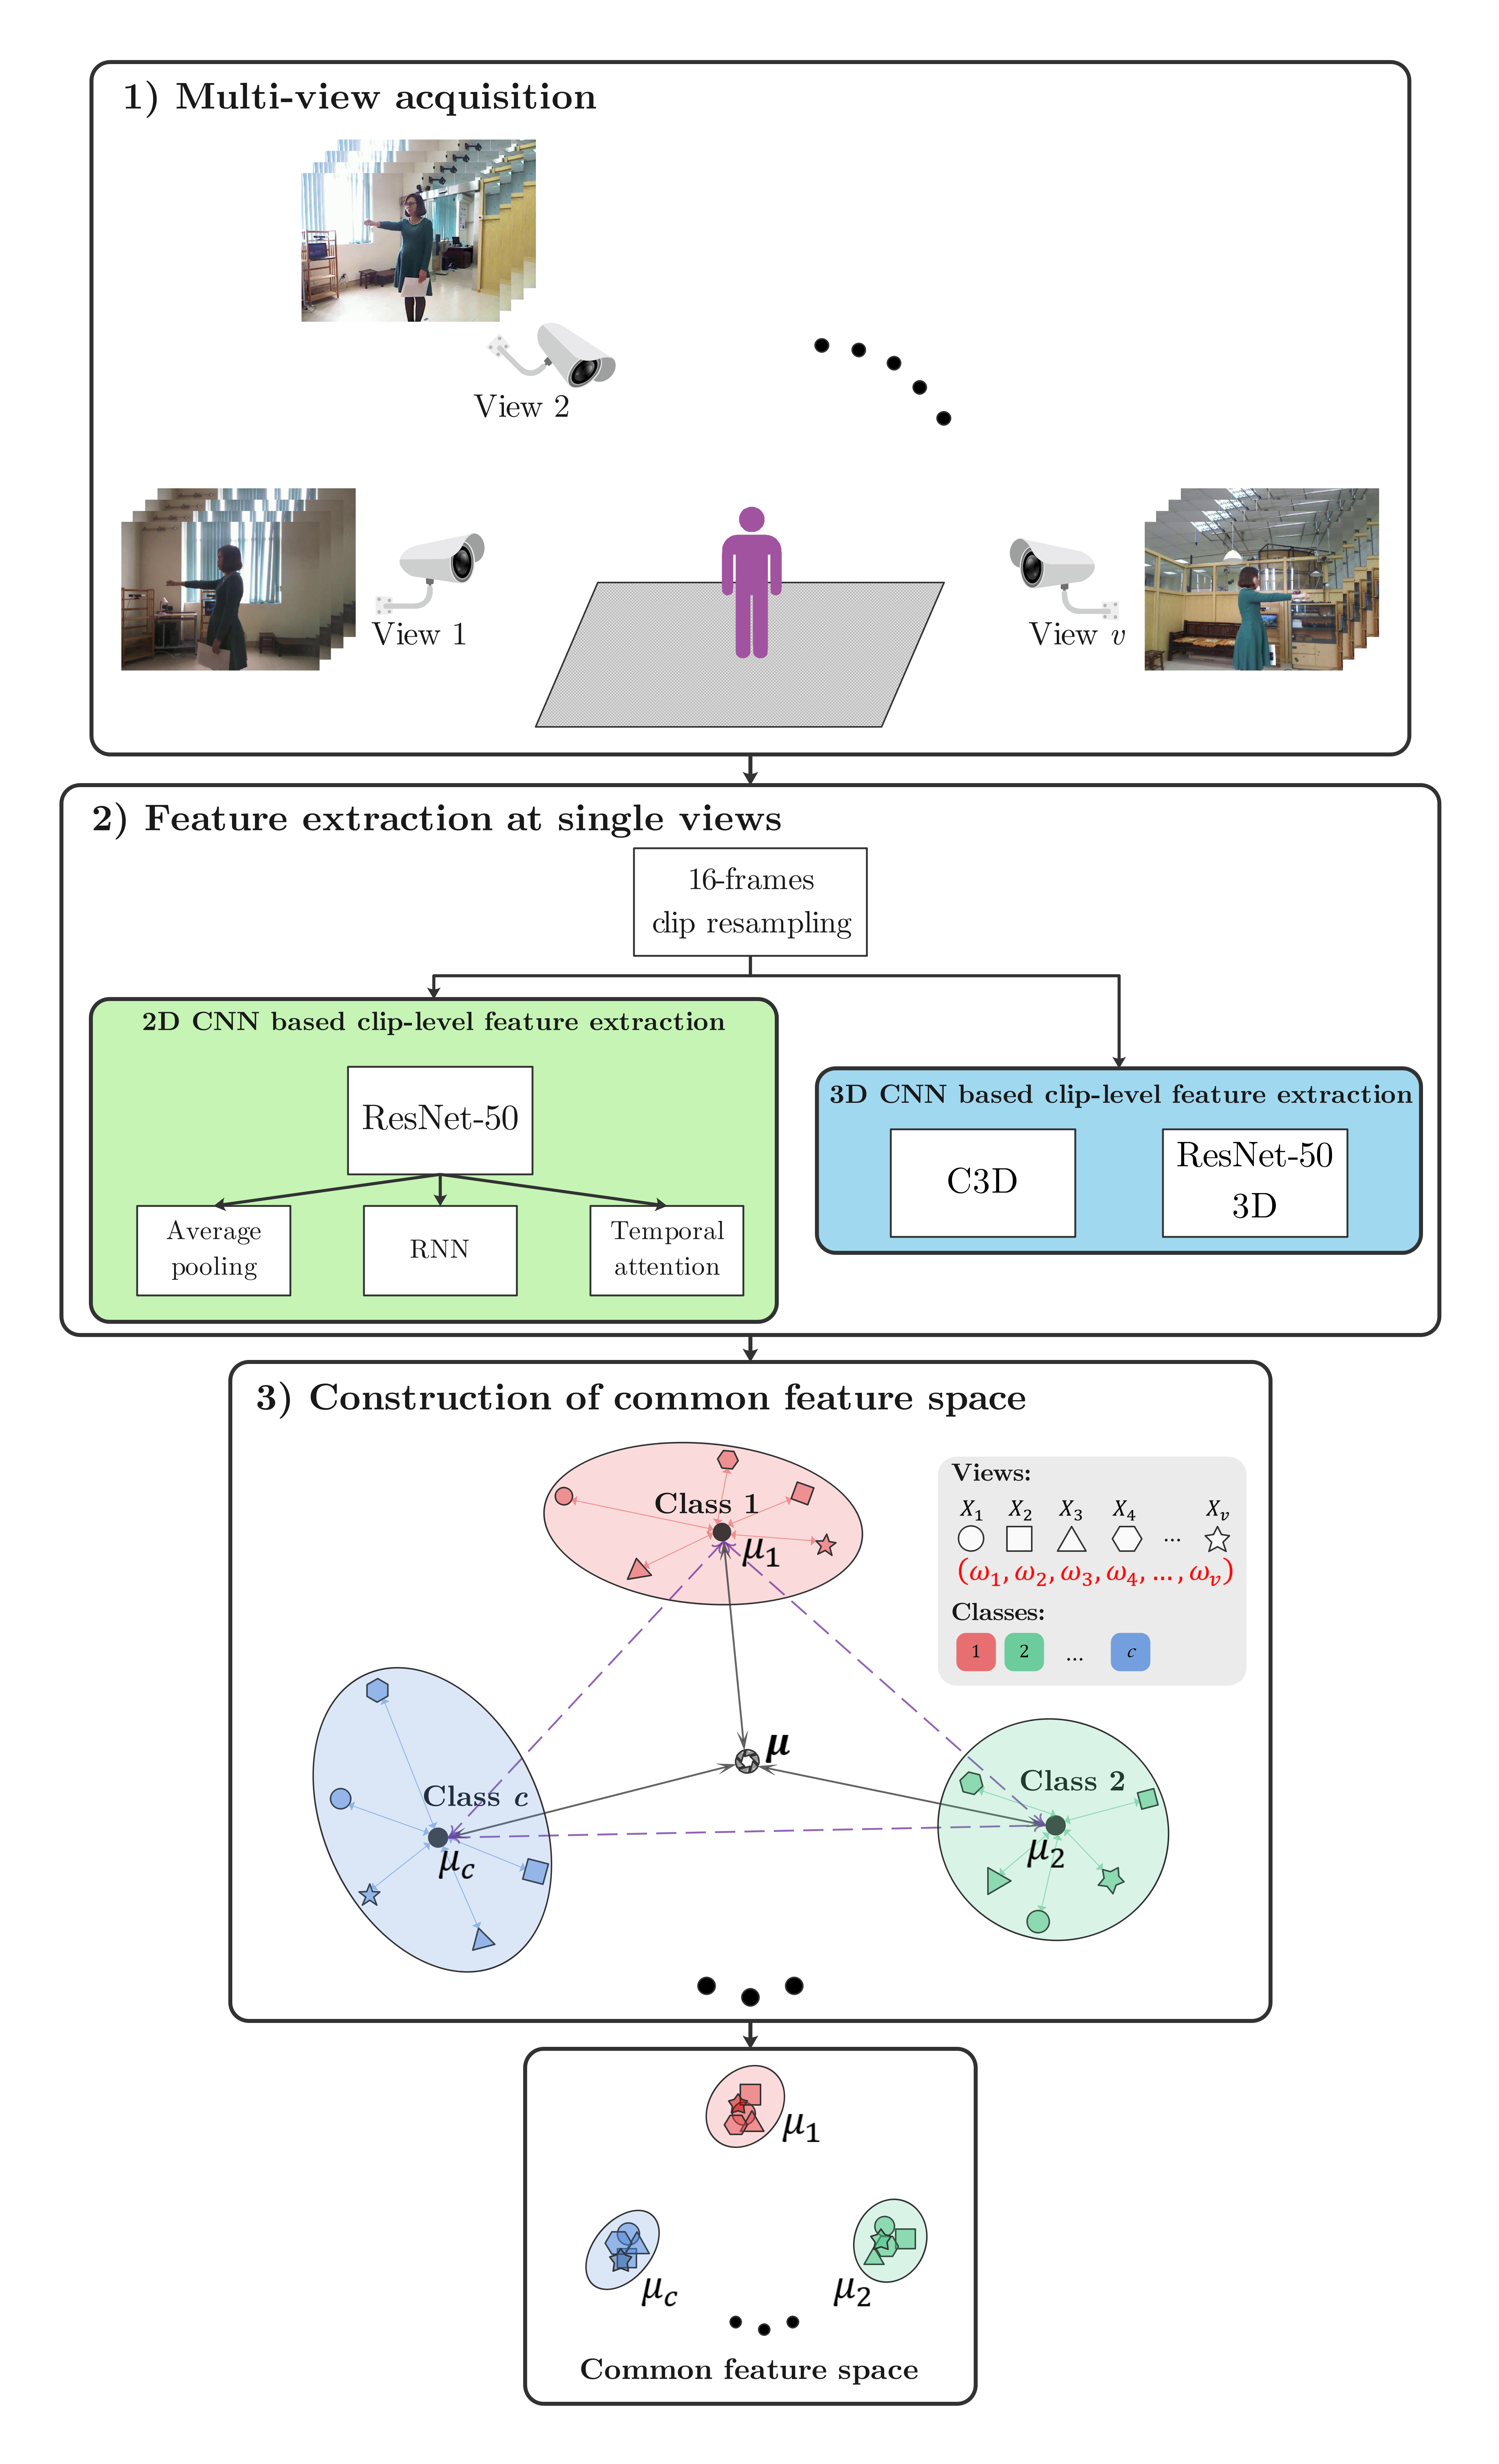
\includegraphics[width=0.85\linewidth]{figs/Framework.png}
        \caption{Proposed framework for building common feature space with pairwise-covariance multi-view discriminant analysis (pc-MvDA).}
        %\vspace{-0.3cm}
        \label{fig:frw}
    \end{figure}
    %In the following, I will detail the step of feature extraction at separated view in subsection \ref{sub:private}, the step of building the common feature space in subsection \ref{sub:common}. 

    %!TEX root = ../../../main.tex

\section{Feature extraction at individual view using deep learning techniques} \label{sec:private}
    %!TEX root = ../../../main.tex

\subsection{2D CNN based clip-level feature extraction}
    First, the ResNet-50 Convolution Neural Network \cite{he2016deep} is used as a 2D CNN network to extract spatial features of each frame in video. Fig.\ref{fig:resnet50} illustrates the architecture of ResNet-50 which composes of five convolutional blocks stacked on top of each other. The network is pre-trained on ImageNet then fine-tuned using training sets described in Section \ref{sec:experimentalresult}. Deep residual features are extracted from the output of the last convolutional block of the network which is a 2048-D feature vector. 
    \begin{figure}[htbp]
        \centering
        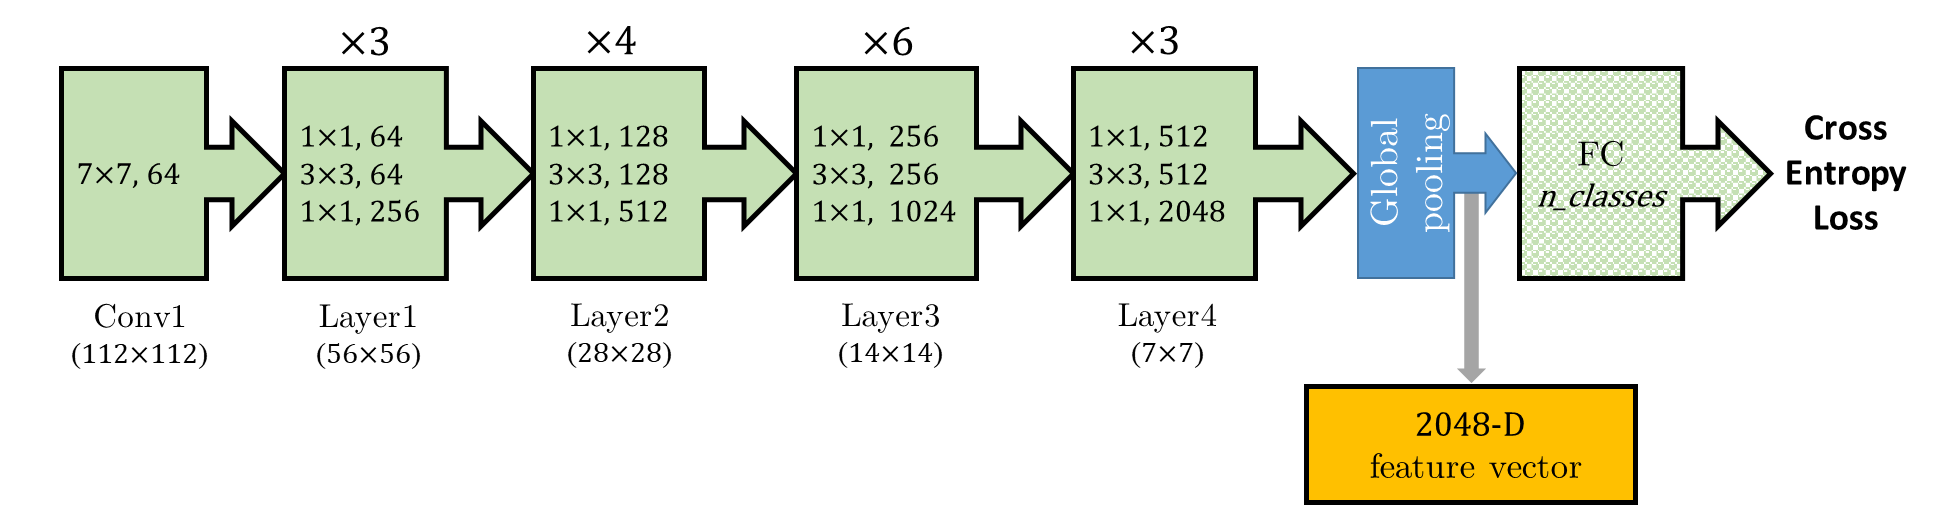
\includegraphics[width=1\linewidth]{Figs/Resnet50.png}
        \caption{Architecture of ResNet-50 utilized in our work for feature extraction at each separated view}
        %\vspace{-0.3cm}
        \label{fig:resnet50}
    \end{figure}
    We then aggregate frame-level features to create video-level features. In this work, we implement three temporal modeling techniques: 1) average pooling (AP); 2) recurrent neural network (RNN) and 3) temporal attention (TA). Fig.\ref{fig:pooling} illustrates three techniques.
    \begin{figure}[htbp]
        \centering
        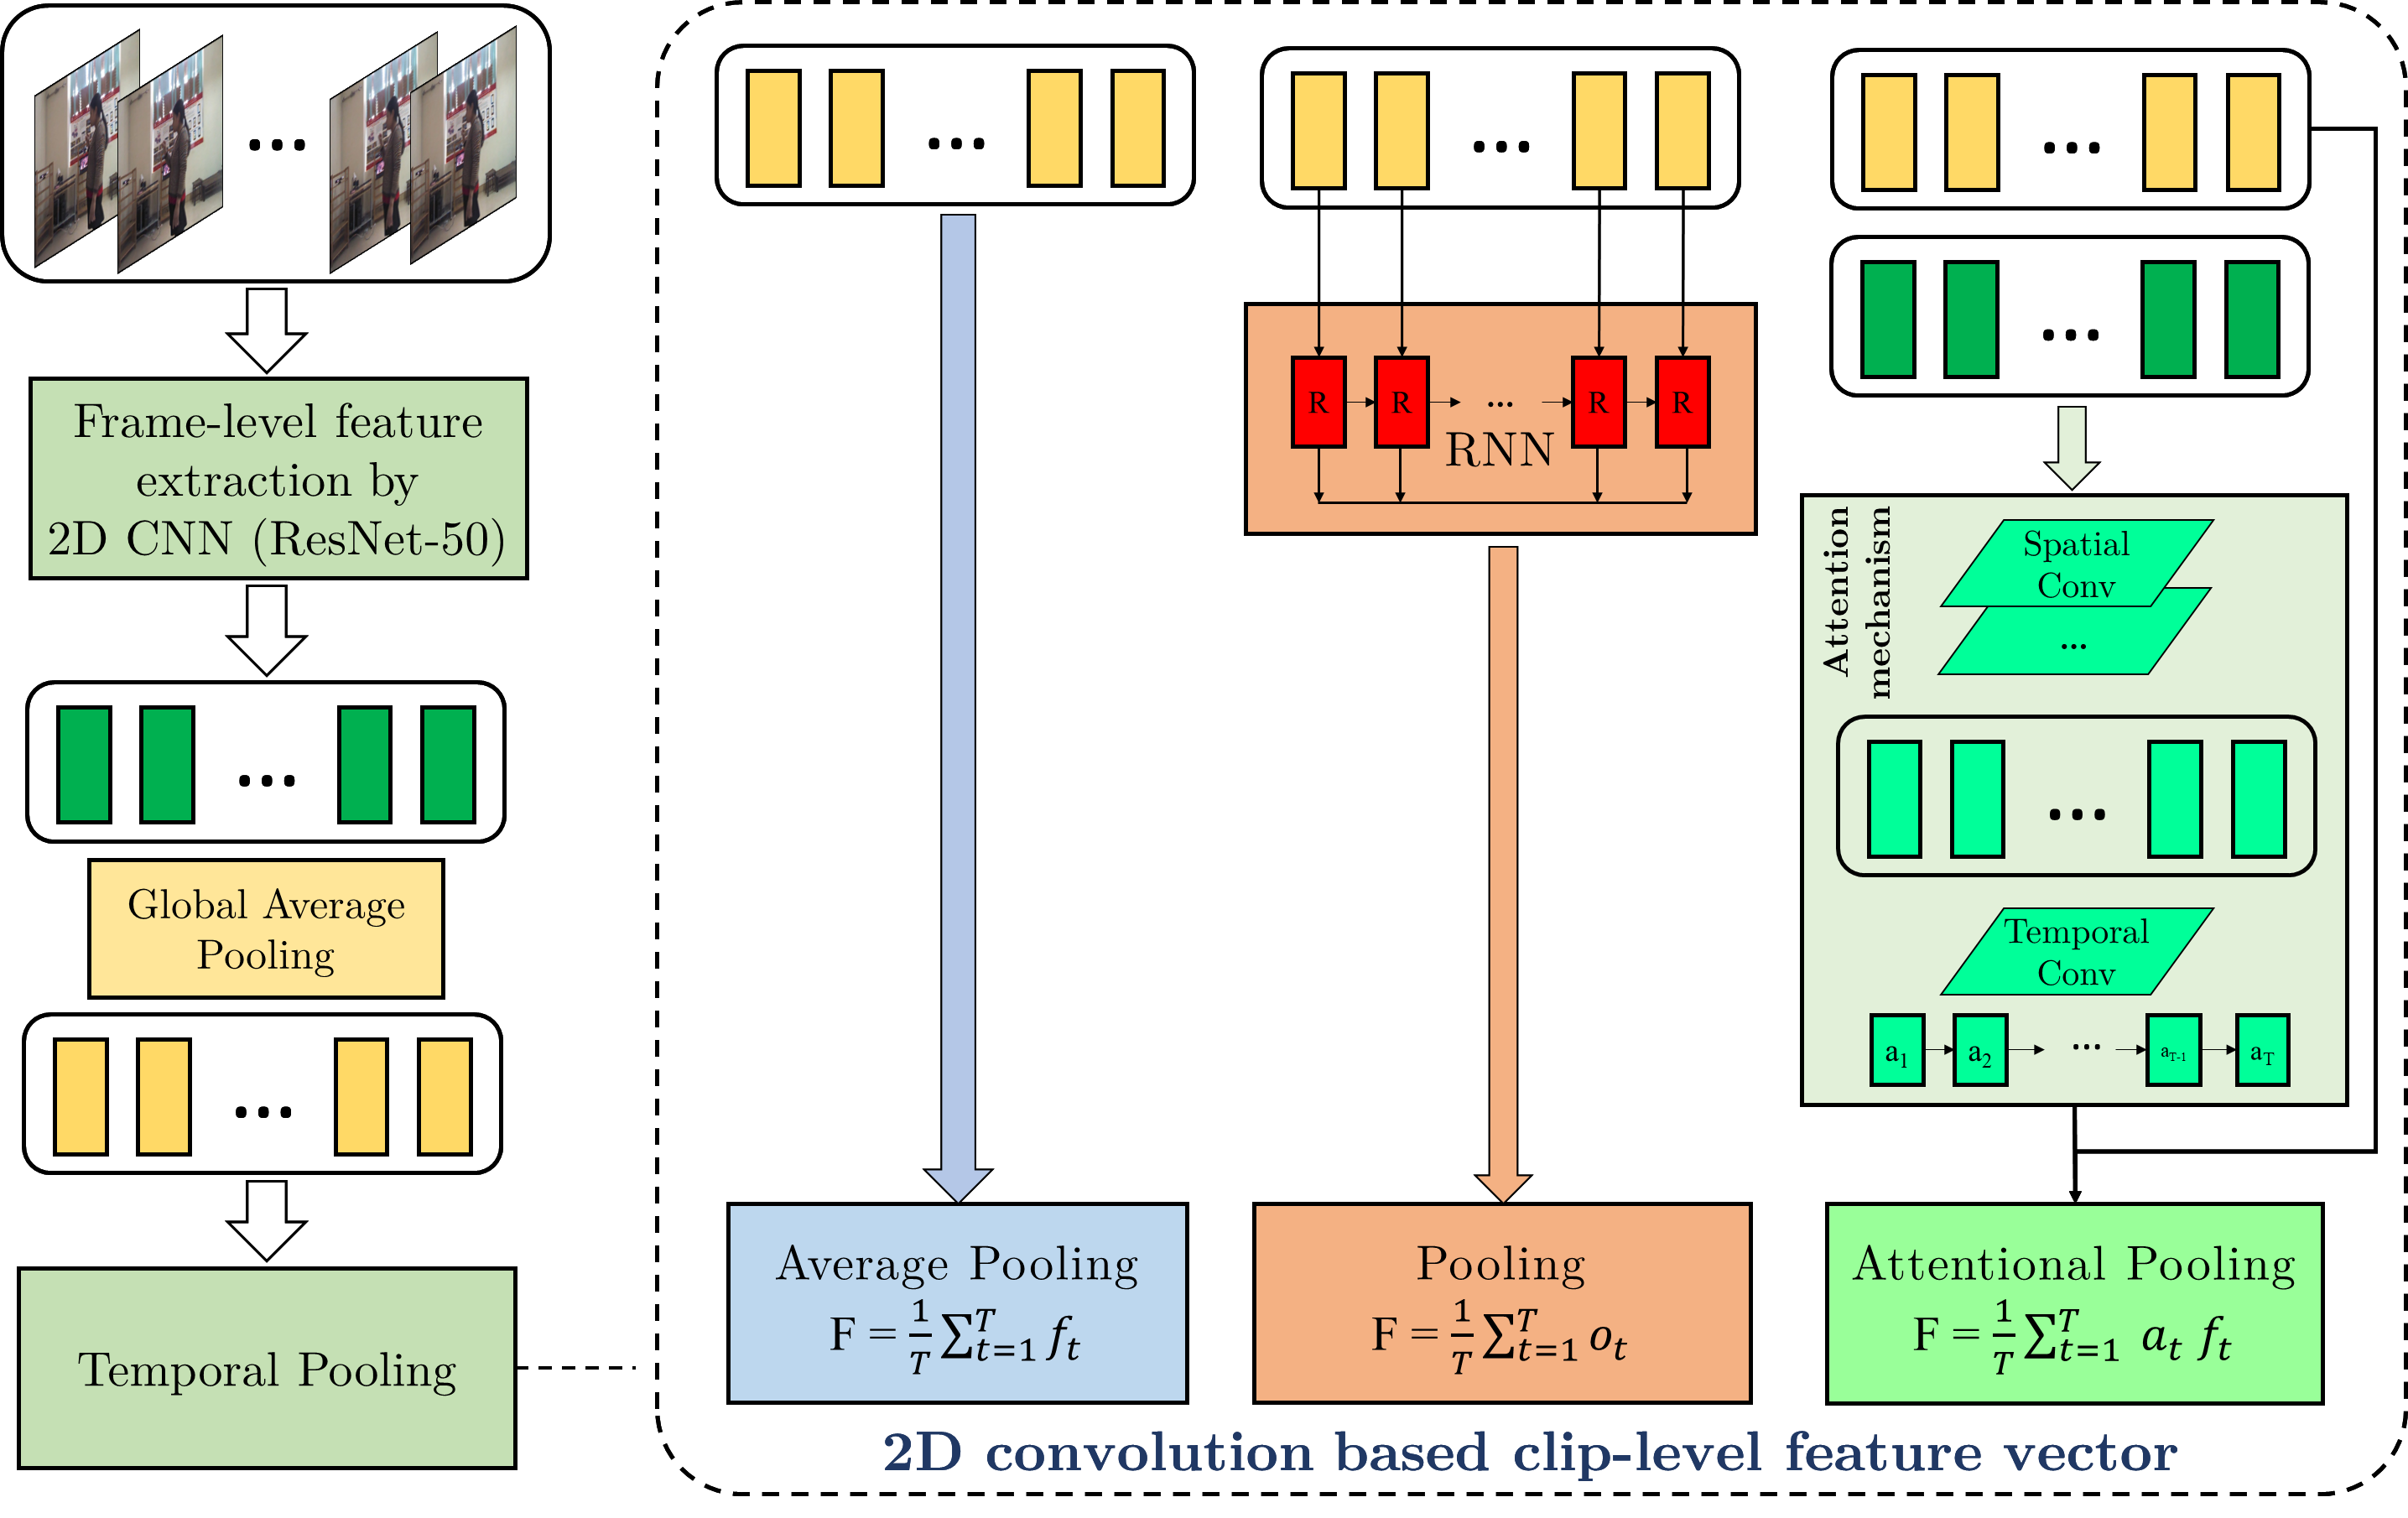
\includegraphics[width=1\linewidth]{Figs/Pooling.png}
        \caption{Three pooling techniques: Average Pooling (AP), Recurrent Neural Network (RNN) and Temporal Attention Pooling (TA)}
        %\vspace{-0.3cm}
        \label{fig:pooling}
    \end{figure}

    \textbf{Average Pooling - AP}: Let ${f}$ be the video-level feature, ${f_t}$ be the frame-level feature at time ${t}$, $T$ be the number of frames in video. Average pooling technique simply averages all frame-level features uniformly to create the video-level feature:
    \begin{equation}
    f=\frac{1}{T}\sum_{t=1}^T{f_t}
    \end{equation}
    As a frame-level feature is a 2048-D vector, the video-level feature is of the same dimension.\\
    \textbf{Recurrent Neural Network - RNN}: An RNN cell encodes a $t^{th}$ frame-level feature at time $t$ of the sequence and passes the hidden state $h_t$ into the next time step. In our work, a cell is a LSTM (Long Short Term Memory). The RNN is a single-layer with $T$ cells. Each cell outputs a 512-D feature vector that contains information of the current frame and the previous ones. We aggregate a sequence of frame-level features into a video-level feature $f$ by calculating the average of the RNN outputs $o_t = R(f_t, o_{t-1})$;$t \in [1;T]$. 
    \begin{equation}
    f=\frac{1}{T}\sum_{t=1}^T{o_t}
    \end{equation}
    \textbf{Temporal Attention - TA}: In the above pooling techniques, frame-level features are equally aggregated. In reality, some frames may have more important roles than remaining ones in recognizing an action. In temporal attention model, we learn a weight $a_t$ for each frame $f_t$ and apply an attention weighted average on the sequence of frame-level features as follows.
    \begin{equation}
    f=\frac{1}{T} \sum_{t=1}^{T}a_{t}f_{t}
    \end{equation}
    To learn the weights $a_t, t \in [1,T]$, we adopt the attention generation network proposed by Jiyang Gao et al. \cite{gao2018revisiting}. The network takes a sequence of frame-level features $[T, w, h, 2048]$, each is tensor extracted from the last convolution layer of ResNet-50. The network architecture consists of two main components: Spatial Convolution and Temporal Convolution. First, a conv layer with shape $\{w,h,2048,d_t\}$ is applied, then we get a $d_t$-dimensional feature for each frame of the clip ($d_t$ = input channel). Then we apply a temporal conv layer $\{3,d_t, 1\}$ on these frame-level features to generate temporal attentions $s_c^t$. Once we have $s_c^t$, the final attention score $a_t$ is computed by Softmax function: 
    \begin{equation}
    a_t = \frac{e^{s_c^t}}{\sum_{k=1}^{T}e^{s_c^k}}
    \end{equation}
    %In all scenarios of pooling, we train the whole net (including a ResNet-50 combined with RNN, TA or AP) on our training set according to the evaluation protocols presented in section \ref{sec:experimentalresult}.

    %!TEX root = ../../../main.tex

\subsection{3D CNN based clip-level feature extraction}
    3D convolution network architectures is increasingly concerned with video based problems. 
    %The main idea of 3D CNN is to utilize 3D convolution operators $(x,y,t)$ instead of 2D operators $(x, y)$, where $x, y$ are spatial dimensions and $t$ is temporal dimension. As a result, 3D CNNs can directly extract video-level features that contain both spatial and temporal information. 
    In this thesis, two 3D CNN architectures are deployed: C3D \cite{duta2017spatio} and ResNet-50 3D \cite{hara2018can}. 

    \textbf{ResNet 3D}: ResNet-50 3D adopts 3D convolution kernels with ResNet-50 architecture. %We apply transfer learning by using Kinetics pre-trained weights \cite{kay2017kinetics}. Like most of the methods presented above, we also get a 2048-dimensional feature vector for each video with input tensor shape $[3, 16, 224, 224]$. They are the number of channels per image (c), the number of frames in the video (s), the width (w) and the height (h) of the frame respectively. 
    The architecture of ResNet-50 3D network is described in the Figure \ref{fig:resnet50_3d}. It has similar architecture as the ResNet-50 but the convolution layers uses 3D operation.  
    \begin{figure}[htbp]
        \centering
        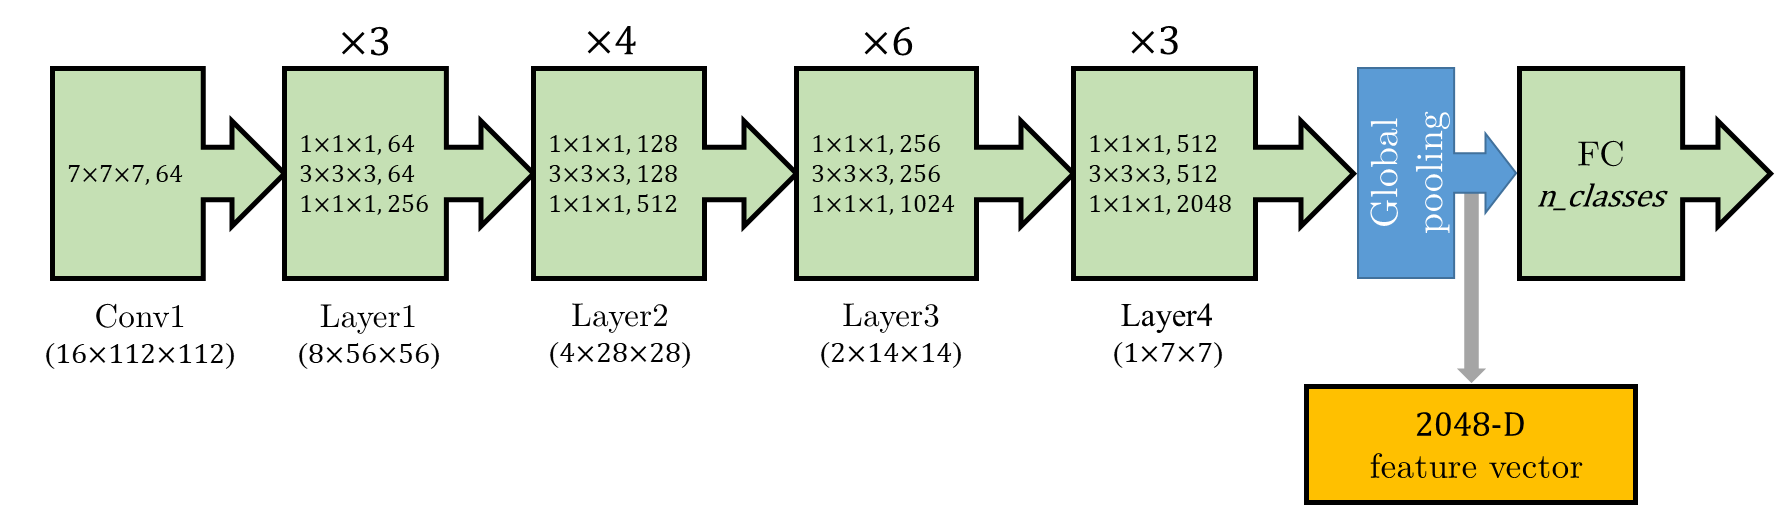
\includegraphics[width=1\linewidth]{Figs/Resnet50_3D.png}
        \caption{Architecture of ResNet-50 3D utilized in this work for feature extraction}
        %\vspace{-0.3cm}
        \label{fig:resnet50_3d}
    \end{figure}

    \textbf{C3D}: 3D deep convolution neural network, which was introduced in \cite{tran2015learning}, has shown to be very efficient for action recognition tasks. C3D takes input as an image sequence instead of a static image, computes the 3D convolution on each 3D cubes from video clip. By doing so, C3D captures both spatial and temporal characteristics of action at the same time.
    \begin{figure}[htbp]
        \centering
        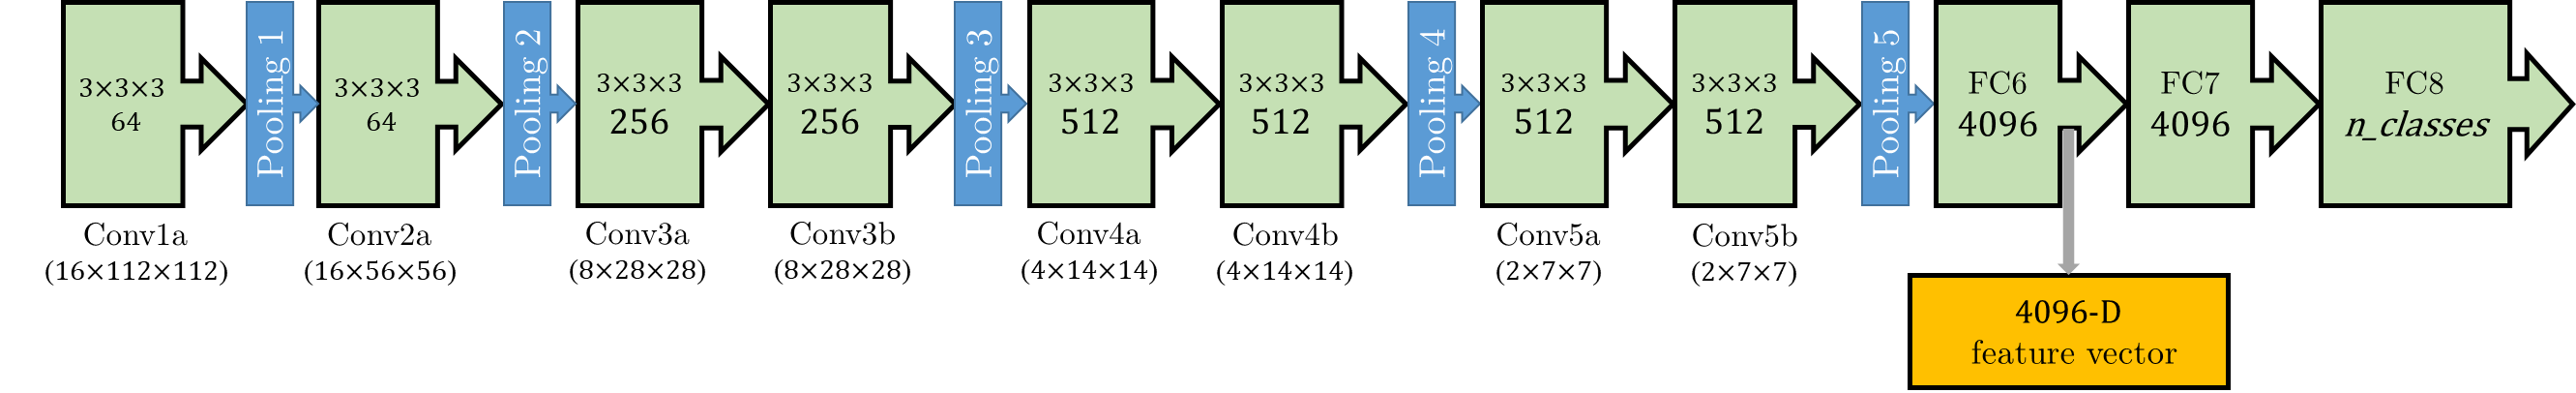
\includegraphics[width=1\linewidth]{Figs/C3D.png}
        \caption{Architecture of C3D utilized in this work for feature extraction}
        %\vspace{-0.3cm}
        \label{fig:C3D}
    \end{figure}
    A C3D network contains 8 convolution, 5 max-pooling and 2 fully connected layers as illustrated in Figure \ref{fig:C3D}. 
    % The number of filters of convolution layers from Conv1 to Conv5 are 64, 128, 256, 512, 512 respectively. All 3D convolution kernels are of size $3\times3\times3$ with stride $1\times1\times1$ and followed by a 3D batch normalization layer. 
    % We utilize the network pre-trained on Sports-1M and fine-tuned on Kinetics dataset.
    The feature vector of 4096 dimensions extracted from FC\-6 layer will be served for training and testing classifiers in further steps.

    To apply in the proposed framework of action and gestures recognition, transfer learning technique is applied for pretrained models on each data stream corresponding to each individual view.
    Details of pre-trained weights and training process of the networks will be presented in Section \ref{sec:experimental_setup}.


    %!TEX root = ../../../main.tex

\section{Construction of common feature space} \label{sec:common}
    %!TEX root = ../../../main.tex

\subsection{Brief summary of Multi-view Discriminant Analysis}
    Suppose that actions belonging to $c$ classes are observed from $v$ views, the number of samples from the $j^{th}$ view of the $i^{th}$ class is $n_{ij}$. We define $X = \{\boldsymbol{x}_{ijk}|i=(1,..,c);j = (1,..,v);k=(1,..,n_{ij})\}$ as samples from $v$ views where 
    $\boldsymbol{x}_{ijk} \in R^{d_j}$ is the $k^{th}$ sample from the $j^{th}$ view of the $i^{th}$ class, $d_j$ is the dimensions of data at the $j^{th}$ view. Here ${\boldsymbol x}_{ijk}$ is a feature vector extracted from the $k^{th}$ sample from the $j^{th}$ view of the $i^{th}$ class. Different methods for features extraction from single view have been presented in previous sections. 

    \textbf{Multi-view discriminant analysis (MvDA)}
    MvDA was an extension of LDA for multi-view scenario \cite{kan2015multi}. It tries to determine a set of $v$ linear transformations to project all action samples from each view $j = (1,..,v)$ to a common space. The projection results of $X$ on the common space is denoted by $Y = \{\boldsymbol{y}_{ijk} = w_j^T\boldsymbol{x}_{ijk}|i=(1,..,c); j=(1,..,v); k=(1,...,n_{ij})\}$. The common space is built by maximizing the between-class variation $\boldsymbol{S}_B^y$ while minimizing the within-class variation $\boldsymbol{S}_W^y$ from all views. $\boldsymbol{S}_B^y$ and $\boldsymbol{S}_W^y$ are computed as follows: 
    \begin{align}
        \boldsymbol{S}_W^y &= \sum_{i=1}^{c}\sum_{j=1}^{v}\sum_{k=1}^{n_{ij}}(y_{ijk}-\boldsymbol{\mu}_i)(y_{ijk}-\boldsymbol{\mu}_i)^T \label{eq:MvDA_Sw}\\
        \boldsymbol{S}_B^y &= \sum_{i=1}^{c}n_i(\boldsymbol{\mu}_i - \boldsymbol{\mu})(\boldsymbol{\mu}_i - \boldsymbol{\mu})^T \label{eq:MvDA_Sb}
    \end{align}
    where $\boldsymbol{\mu}_i=\frac{1}{n_i}\sum_{j=1}^{v}{\sum_{k=1}^{n_{ij}}}{\boldsymbol{y}_{ijk}}$ is the mean of all samples of the $i^{th}$ class from all views in the common space; $\boldsymbol{\mu}=\frac{1}{n}\sum_{i=1}^{c}\sum_{j=1}^{v}{\sum_{k=1}^{n_{ij}}{\boldsymbol{y}_{ijk}}}$ is the mean of all samples of all classes from all views in the common space; $n=\sum_{i=1}^{c}n_i$ is the total data samples from all views.
    Then the objective function is formulated by a Rayleigh quotient:
    \begin{equation}
        (\boldsymbol{\omega}_1^*,\boldsymbol{\omega}_2^*, ..., \boldsymbol{\omega}_v^*) = \operatorname*{argmax}_{\boldsymbol{\omega}_1, \boldsymbol{\omega}_2,..., \boldsymbol{\omega}_v}\frac{trace({S}_B^y)}{trace({S}_W^y)}
        \label{eq:MvDA}
    \end{equation}
    According to \cite{kan2016multi}, the optimization problem could be analytically solved through generalized eigenvalue decomposition. 

    %\textbf{Multi-view discriminant analysis with view consistency (MvDA-vc):}
     In \cite{kan2016multi}, the authors observed that as multiple views correspond to the same objects, there should be some correspondence between multiple views. They then introduce a view consistency constraint into the objective function. The method is called as MvDA-vc. In this paper, we will also compare with MvDA-vc but our method improves the MvDA, so we will not detail MvDA-vc in this section. 
     
     %According to the experimental results presented in the next section, MvDA-vc helps to improves significantly performance of recognition. However, it is difficult to explain explicitly and intuitively how view consitency helpts
     
    %  , that means if $\boldsymbol{X}_j, \boldsymbol{X}_r$ are observed at $j^{th}$ and $r^{th}$ views, then there exists a certain transformation $\boldsymbol{R}$ such that $\boldsymbol{X}_j = \boldsymbol{R}\boldsymbol{X}_r$. As a result, the transformations obtained from two views (i.e. the projection of features extracted from singe view to common view) should have similar relationship: ${\omega}_j = \boldsymbol{R}{\omega}_r$. Let us define $\beta_i$ that captures the structure of the transformation ${\omega}_i$. Then the $\beta_j$ and $\beta_r$ capturing the structures of two transformations of two views $j$ and $r$ should be identical ${\beta}_j = {\beta}_r$.
     
    %  Generalizing to $v$ views, suppose that ${\boldsymbol\beta}_j, j=(1,..,v)$ captures the structures of $v$ transformations ${w}_j$. Following the above observation, the $\boldsymbol{\beta}_r, r=(1,..,v)$ should resemble mutually. That means the similarity between the pair of $\boldsymbol{\beta}_j$ and $\boldsymbol{\beta}_r$ should be minimized. 
    % \begin{equation}
    %      \sum_{j,r=1}^{v}||\boldsymbol{\beta_j} - \boldsymbol{\beta_r}||_2^2
    % \end{equation}
    %  This term is called in \cite{kan2016multi} {\itshape view consistency} and will be added to the denominator of Eq.\eqref{eq:MvDA}
    % \begin{equation}
    % \small
    %     (\boldsymbol{\omega}_1^*,\boldsymbol{\omega}_2^*, ..., \boldsymbol{\omega}_v^*) = \operatorname*{argmax}_{\boldsymbol{\omega}_1, \boldsymbol{\omega}_2,..., \boldsymbol{\omega}_v}\frac{trace({S}_B^y)}{trace({S}_W^y) + \alpha\sum_{j,r=1}^{v}||\boldsymbol{\beta_j} - \boldsymbol{\beta_r}||_2^2} 
    %     \label{eq:MvDA-vc}
    % \end{equation}
    % Similarly, this optimization problem could be analytically solved by relaxing to the ratio trace problem as Eq.\eqref{eq:MvDA}. In the Eq.\eqref{eq:MvDA-vc}, $\alpha$ is an empirically chosen parameter. It puts a weight on the view-consistency assumption. When $\alpha = 0$, the MvDA-vc becomes the original MvDA. 

    %!TEX root = ../../../main.tex

\subsection{Pairwise-covariance Multi-view Discriminant Analysis pc-MvDA}
    MvDA emphasizes on finding a common space with minimal within-class variation while the distances between class means and global mean are jointly maximized. However, the distances between some pairs of classes can be disregarded. In this paper, to obtain this property, we modified MvDA with reformulated between and with-in class scatter matrices terms in a pairwise manner. First, let us define a new inter-class scatter matrix formula that takes paired distance into account:
    \begin{equation}
        \boldsymbol{S}_B^y=\sum_{a=1}^{c}\sum_{b=a+1}^{c}{\left(\mu_a-\mu_b\right)\left(\mu_a-\mu_b\right)^T}
    \end{equation}
    where $a$, $b$ are two distinct classes. For each pairs of class $a$ and class $b$, the between covariance is calculated as:
    \begin{equation}
        {\boldsymbol{S}_B^y}_{ab}={\left(\mu_a-\mu_b\right)\left(\mu_a-\mu_b\right)^T}
        \label{eq:Sb_ab}
    \end{equation}

    The intra-class scatter matrix $\boldsymbol{S}_W^y$ of MvDA is calculated as simple summation of all covariance matrices of each $i^{th}$ class, $i = {1,...,c}$:
    \begin{equation}
        {\boldsymbol{S}_W^y}_i=\sum_{j=1}^{v}\sum_{k=1}^{n_{ij}}{\left(y_{ijk}-\mu_i\right)\left(y_{ijk}-\mu_i\right)^T}
    \end{equation}

    Mathematically, it assumes data samples from each class among all views are identically Gaussian distributed, and contribute evenly to the minimization of intra-class scatter. In reality, it is hardly the case as data variations of samples from different classes and different view points are usually drastically diverse and may also have different dimensions.

    To better represent the distribution of data, pc-MvDA uses a paired intra-scatter matrix which is denoted as
    \begin{equation}
        {\boldsymbol{S}_W^y}_{ab}=\beta\frac{n_a{\boldsymbol{S}_W^y}_a+n_b{\boldsymbol{S}_W^y}_b}{n_a+n_b}+\left(1-\beta\right){\boldsymbol{S}_W^y}
        \label{eq:Sw_ab}
    \end{equation}
    where $0\le\beta\le1$ is a hyper-parameter for regularization between the original global intra-covariance ${\boldsymbol{S}_W^y}$ and the novel two local class covariances ${\boldsymbol{S}_W^y}_a$ and ${\boldsymbol{S}_W^y}_b$. This formulation is closer to the value of covariances of both classes than the standard intra-covariance.

    Instead of solving the vanilla generalized eigen value problem for the whole dataset, we split it into sub-problems for each pairs of class $a$ and $b$, in which we define the objective distance to be minimized between two corresponding classes.
    \textbf{Difference of our proposed method compared to pairwise LDA (pc-LDA)}
    In pc-LDA \cite{kong2014pairwise}, the pairs of $a$ and $b$ classes are regarded as two Gaussian distributions $\mathcal{N}_a(\mu_a,{\boldsymbol{S}_W^y}_a), \mathcal{N}_b(\mu_b,{\boldsymbol{S}_W^y}_b)$ and the objective distance between two classes is defined as their Kullback-Leibler divergence \cite{kullback1951}:
    \begin{equation}
        D_{KL}\left(\mathcal{N}_a\parallel\mathcal{N}_b\right)=\frac{1}{2}\left(\mu_a-\mu_b\right)^{T}{\left({\boldsymbol{S}_W^y}_{ab}\right)}^{-1}\left(\mu_a-\mu_b\right),
    \end{equation}
    Then the final objective is properly weighted to focus on classes with more samples:
    \begin{equation}
        \operatorname*{min}_{\boldsymbol{\omega}_1, \boldsymbol{\omega}_2,...,
        \boldsymbol{\omega}_v}{J}=\sum_{a=1}^{c}\sum_{b=a+1}^{c}{\frac{n_an_b}{{[2D_{KL}\left(\mathcal{N}_a\parallel\mathcal{N}_b\right)]}^q}}
        \label{eq:pc-LDA}
    \end{equation}
    here $q\ge1$ is a hyper-parameter that controls how much the pairs of classes with smaller objective distances are biased over the others.

    In our observation, the minimization of KL divergence for each pairs of classes $a$ and $b$ can be substituted by a generalized eigenvalue problem with the pairwise ${\boldsymbol{S}_W^y}_{ab}$ and the ${\boldsymbol{S}_B^y}_{ab}$ we defined. Although these sub-problems do not have an unified analytical solution to be solved concurrently, the criteria can be formulated in various differentiable ways like in \cite{fukunaga1990441} so we can use gradient descent algorithm:
    \begin{equation}
        J_1=\frac{tr(S_B)}{tr(S_W)};\quad 
        J_2=tr\left(\frac{S_B}{S_W}\right);\quad
        J_3=tr\left|\left|\frac{S_B}{S_W}\right|\right|;\quad
        J_4=\frac{det(S_B)}{det(S_W)}
    \end{equation}

    We choosed the former Fisher loss as the ratio of scalar values is computationally cheaper. Comparing to the objective of pc-LDA in Eq.\eqref{eq:pc-LDA}, our proposed model is obviously more efficient since it contains only simple operators and the need to inverse a singular-prone matrix is negated. Therefore, it is better fit in the scenario where we want to train the model multiple iterations over multi-view high dimensional output.

    Our final objective function of pairwise-covariance multi-view discriminant analysis is sum of all pairwise Fisher criteria with normalized weights:
    \begin{equation}
        \operatorname*{min}_{\boldsymbol{\omega}_1, \boldsymbol{\omega}_2,..., \boldsymbol{\omega}_v}{J}=\sum_{a=1}^{c}\sum_{b=a+1}^{c}{\frac{n_an_b}{n_{cc}^2}{\left[{\frac{trace\left({\boldsymbol{S}_W^y}_{ab}\right)}{trace\left({\boldsymbol{S}_B^y}_{ab}\right)}}\right]}^{q}}
        \label{eq:pc-MvDA}
    \end{equation}
    where $n_{cc}$ is the number of common components as coined in \cite{you2019multi} or simply number of samples in each view. This added normalization term assures that the objective does not depend on size of dataset.

    Let's look at the Fig.\ref{fig:frw}, the nominator of MvDA(-vc) $\boldsymbol{S}_B^y$ is the sum of all distances from mean of every class $\mu_i$, $i = {1,...,c}$ to the mean of all classes $\mu$. This helps to push class far away from the mean of all classes (the dotted green lines in Fig.\ref{fig:frw}). However, it may not ensure that the classes will be far from each other (Fig.\ref{fig:pc-MvDA}a). In this work, we take the pairwise distance into account and integrate them in an multi-view framework (the dotted violet lines in Fig.\ref{fig:frw}). Thanks to this, the classes will be more discriminated (Fig. \ref{fig:pc-MvDA}b). The algorithm for solving pc-MvDA is presented in supplemental materials. 

    \textbf{Illustrative examples:} We illustrate the advantage of pc-MvDA on artificial datasets. Firstly, using function provided by scikit-learn library, we generate several isotropic Gaussian blobs equal to desired number of classes as data samples from one single view. To generate other views, we clone and apply translation, point-wise noise and rotation with random orthogonal group multiplication to the first view.

    In Fig.\ref{fig:synthetic1}, MvDA and pc-MvDA results on 2D synthetic dataset of 180 data points in 2-D space. There are three classes, observed at three viewpoints. We show data distribution and 1-D projection results using MvDA and pc-MvDA respectively. We notice that data points of two classes (the first and the third classes) are close together in original space. When we project in common space by MvDA, these classes are still close together. In contrast, these classes are more discriminant when projected by pc-MvDA.

    Similar to the first example, in the second example, we generate 300 data points of 5 classes observed from 3 different views (Fig.\ref{fig:synthetic2}). We observe that the five clusters of pc-MvDa common space contract strongly and become more separated as compared to the MvDA results (especially the first and the fourth classes).

    \begin{figure}[htbp]
        \centering
        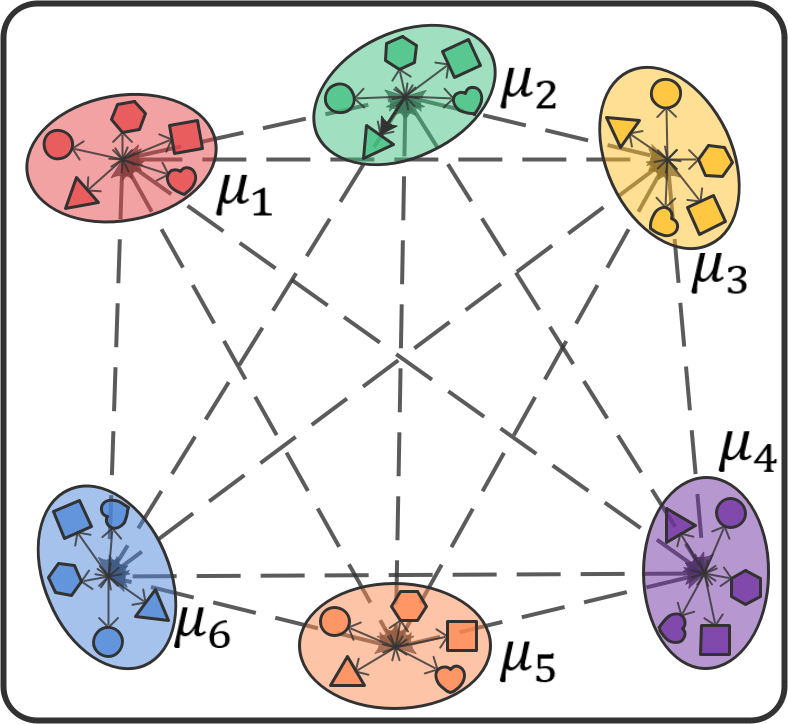
\includegraphics[width=0.7\linewidth]{Figs/pc-MvDA.png}
        \caption{a) MvDA does not optimize the distance between paired classes in common space. b) pc-MvDA takes pairwise distances into account then distinguish better the classes.}
        %\vspace{-0.3cm}
        \label{fig:pc-MvDA}
    \end{figure}

    \begin{figure}[htbp]
        \centering
        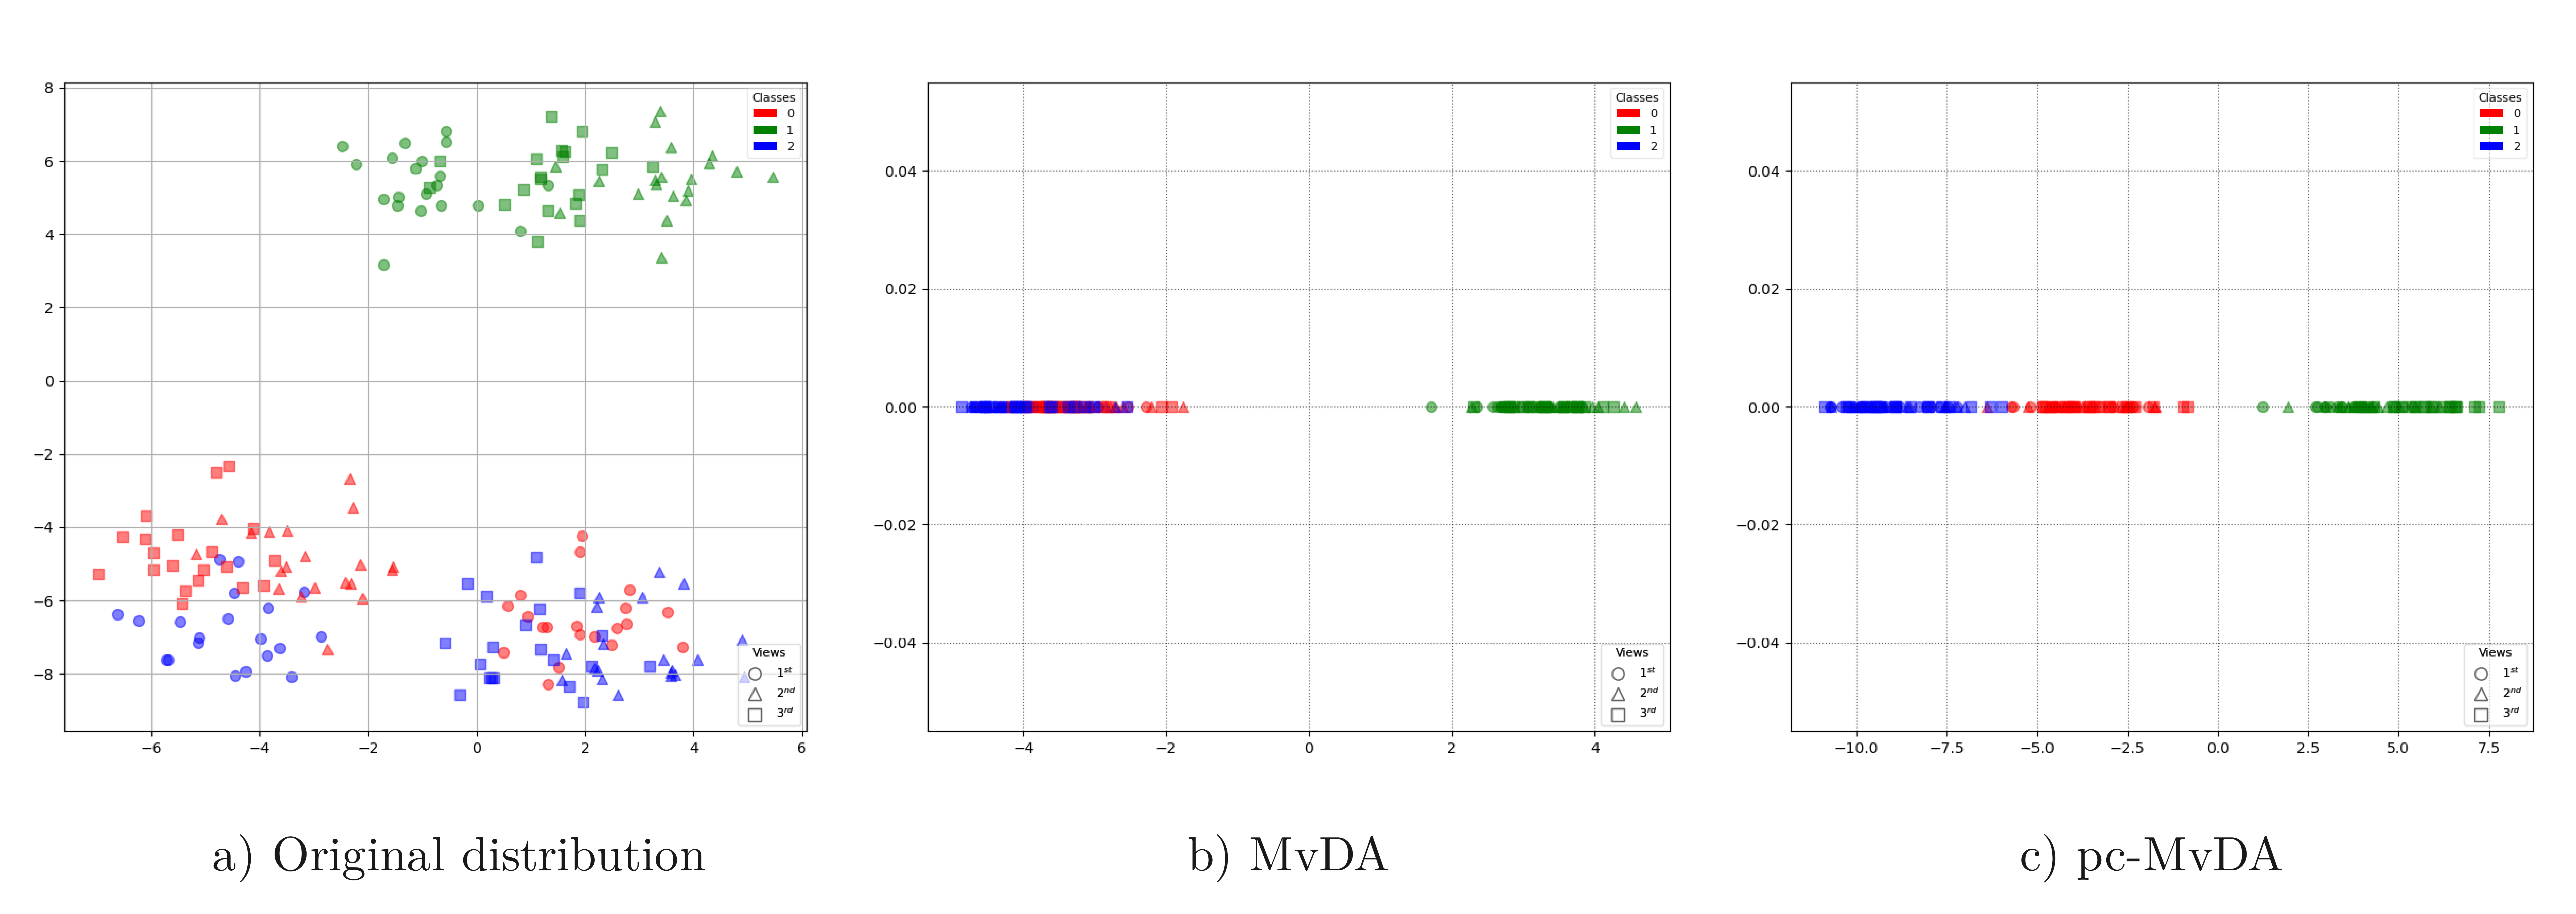
\includegraphics[width=1\linewidth]{Figs/Synthetic1.png}
        \caption{A synthetic dataset of 180 data points, evenly distributed to 3 classes among 3 different views; a) 2-D original distribution; b) 1-D projection of MvDA; c) 1-D projection of pc-MvDA}
        %\vspace{-0.3cm}
        \label{fig:synthetic1}
    \end{figure}

    \begin{figure}[htbp]
        \centering
        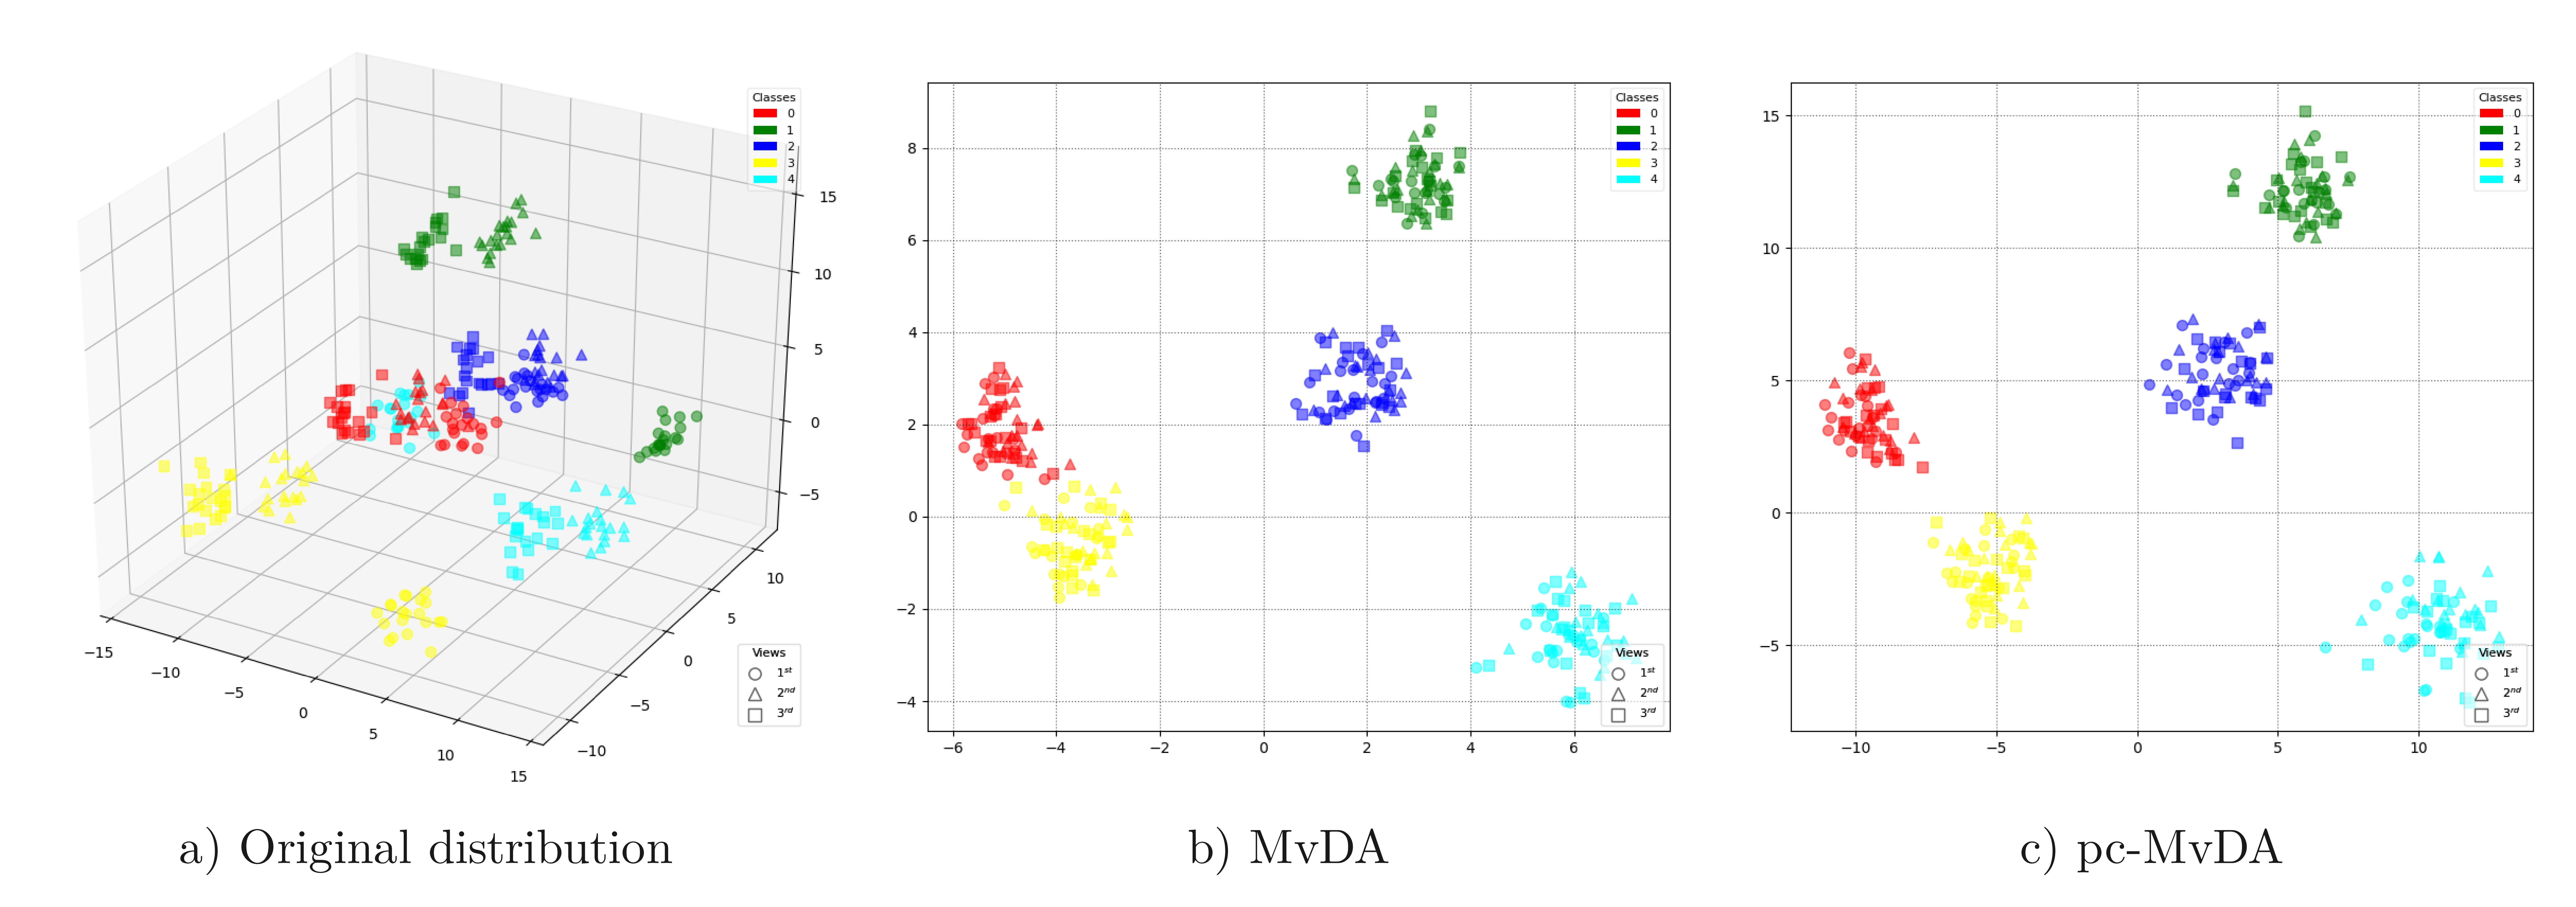
\includegraphics[width=1\linewidth]{Figs/Synthetic2.png}
        \caption{A synthetic dataset of 300 data points, evenly distributed to 5 classes among 3 different views; a) 3-D original distribution; b) 2-D projection of MvDA; c) 2-D projection of pc-MvDA}
        %\vspace{-0.3cm}
        \label{fig:synthetic2}
    \end{figure}



    \section{Summary}
        The novel human action and gesture recognition framework was introduced in this chapter, which consists of two components.
        Firstly, convolutional based clip-level extraction using either 2D CNN (i.e. ResNet) combined with temporal modeling techniques (AP, RNN, TA) or 3D CNN (i.e. C3D, ResNet 3D) are trained separately for each view.
        In the later stage, multi-view analysis algorithms (including pc-MvDA - the main contribution of this thesis) are employed to project common features space, in which the final classification process take place.
        The new formulation of pc-MvDA successfully enforces class separability by adding pairwise distance constraint and casting the final objective to an efficient gradient descent optimization problem that can theoretically be backpropagated to previous layers of CNN feature extractors.
        However, the framework is currently not easily end-to-end trainable due to enormous size of multiple deep feature extractors coupled with the problematic prerequisite of knowing class means when using multi-view analysis as loss function.

    %!TEX root = ../../main.tex

\chapter{Experiments} \label{chap:experimental_result}
    \section{Introduction}
        This chapter represents the methodology proposed in this thesis.
        In section \ref{sec:datasets} and section \ref{sec:protocol}, the benchmarking datasets and evaluation protocol used in experiments of this thesis will be listed out.
        Section \ref{sec:experimental_setup} gives details about the programming configurations of the experiments.
        And finally, section \ref{sec:results} shows the experimental outcomes of proposed framework, compares them with results reported in existing publications and gives discussion.

    %!TEX root = ../../../main.tex

\section{Datasets} \label{sec:datasets}

    In this thesis, three datasets are used in evaluation of the proposed algorithm. Two of which are benchmark datasets IXMAS \cite{weinland2006free}, MuHAVi \cite{murtaza2016multi} and the other (namely MICAGes) is recorded at computer vision department of MICA Institute. 

    %!TEX root = ../../../main.tex

\subsection{IXMAS dataset}
    The IXMAS dataset is a multi-view dataset built by Perception project \cite{weinland2006free}.
    It contains 12 action classes (check watch, cross arms, scratch head, sit down, get up, turn around, walk, wave, punch, kick, point and pick up) recorded simultaneously by 5 cameras (4 side view cameras and 1 top view camera).
    Each action is performed 3 times by 10 actors (5 males / 5 females).
    Some representative frames of action \textit{check watch} are shown in Fig.\ref{Fig:IXMAS1}.

    \begin{figure}[h]
        \centering
        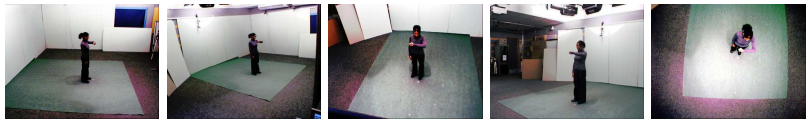
\includegraphics[width=1\linewidth]{figs/IXMAS1.png}
        \caption{Illustration of frames extracted from action \textit{check watch} observed from five camera viewpoints.}
        %\vspace{-0.3cm}
        \label{Fig:IXMAS1}
    \end{figure}

    During the time of writing this thesis, the original version of the dataset is no longer publicly available due to the privacy issues.
    Only a subset of 1692 samples containing samples from four side camera views (excluding the top down view) that have been downloaded previously was utilized with the agreement of the data-set's authors.
    The comparison with SOTA methods on this dataset will only be taken from the four side view cameras. 

    %!TEX root = ../../../main.tex

\subsection{MuHAVi dataset}
    The MuHAVi dataset is constructed and introduced by \cite{murtaza2016multi}. It is usually referred as MuHAVi-uncut because it contains full, raw videos of 17 actions, asynchronously captured by eight cameras that provide completely overlapping coverage of a rectangular action zone from different viewing directions as in Fig.\ref{Fig:MuHAVi1}. 

    \begin{figure}[h]
        \centering
        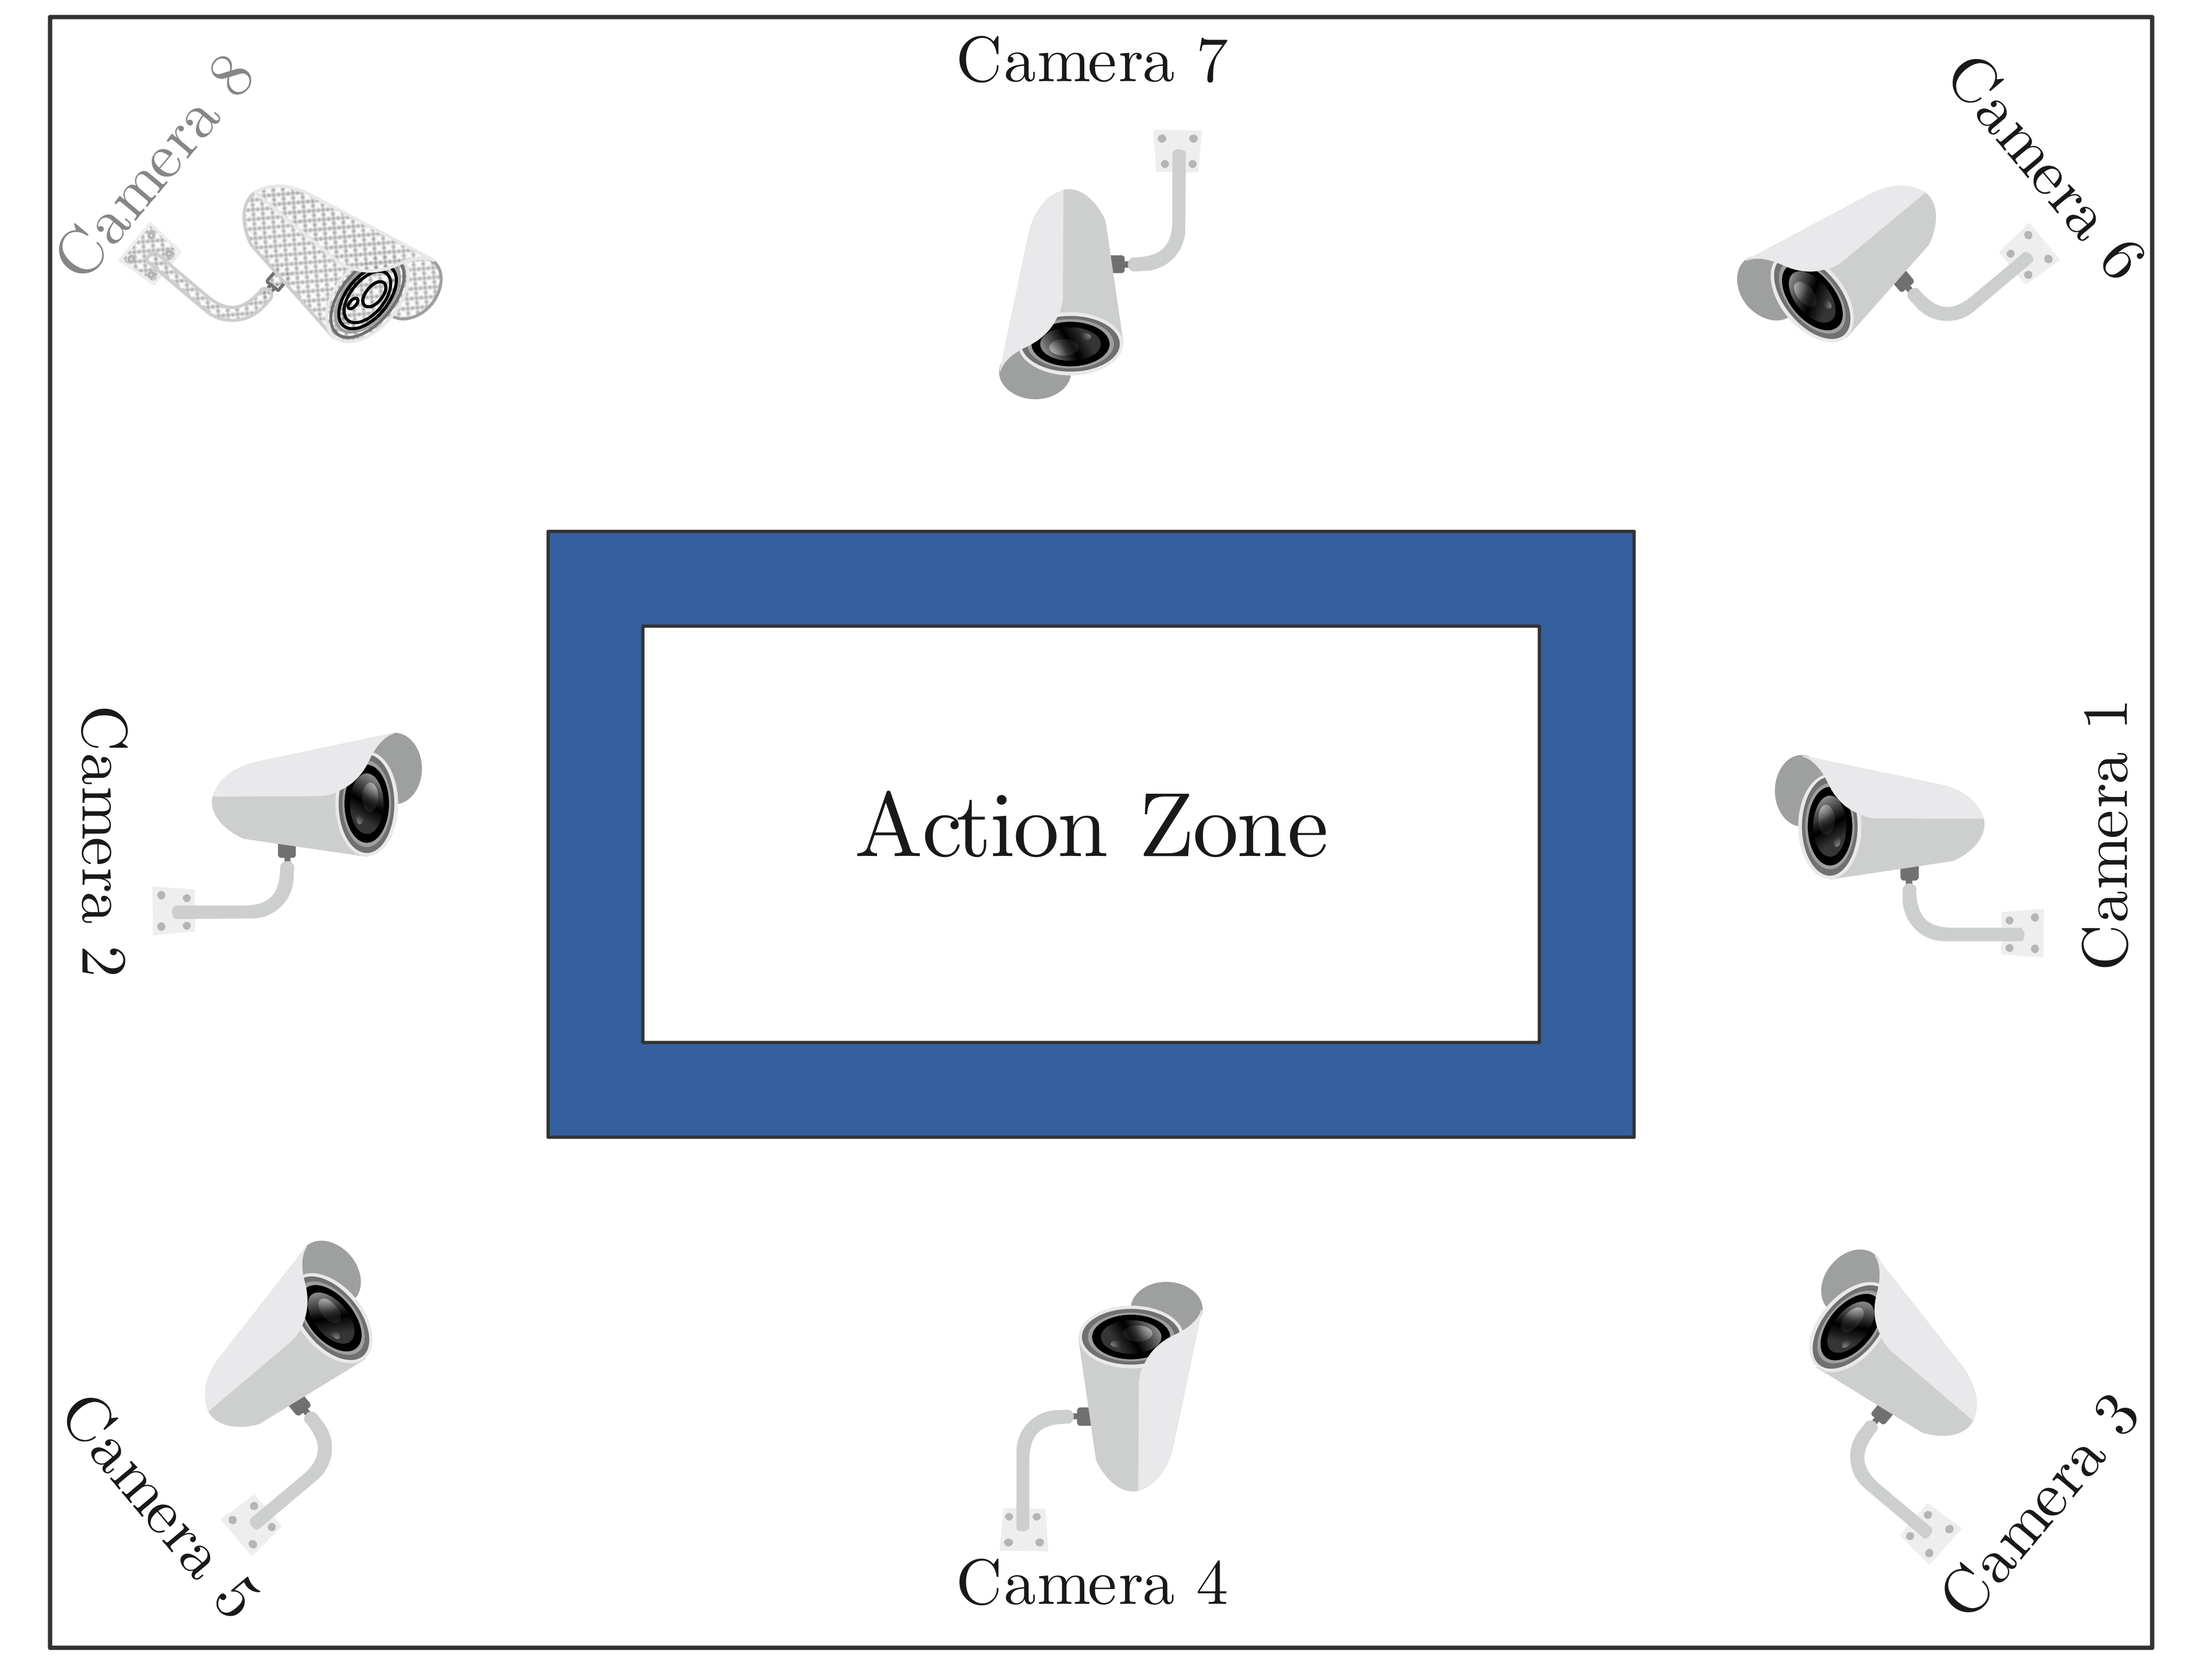
\includegraphics[width=0.8\linewidth]{figs/MuHAVi1.png}
        \caption{Environment setup to collect action sequences from 8 views \cite{murtaza2016multi}.}
        %\vspace{-0.3cm}
        \label{Fig:MuHAVi1}
    \end{figure}

    The actions are are walk turn back, run stop, punch, kick, shotgun collapse, pull heavy object, pickup throw object, walk fall, look in car, crawl on knees, wave arms, draw graffiti, jump over fence, drunk walk, climb ladder, smash object, and jump over gap. 
    Each was performed several times by 7 actors (5 males / 2 females). 
    The videos were collected at rate of 25 fps with resolution of 720 $\times$ 576, except for the $8^{th}$ camera whose data is not included in experiments of this thesis due to absence of annotation.
    Some representative frames of action \textit{punch} are shown in Fig.\ref{Fig:MuHAVi2}.

    \begin{figure}[htbp]
        \centering
        \includegraphics[width=1\linewidth]{figs/MuHAVi2.png}
        \caption{Illustration of frames extracted from an action \textit{punch} observed from Camera 1 to Camera 7.}
        %\vspace{-0.3cm}
        \label{Fig:MuHAVi2}
    \end{figure}

    %!TEX root = ../../../main.tex

\subsection{MICAGes dataset}
    There does not exist a dataset publicly available in the literature which is dedicated to the evaluation of robustness of hand gesture recognition w.r.t. viewpoint changes.
    Therefore, thanks to the work of computer vision department at MICA Institute, a dataset was carefully designed and collected from multiple viewpoints in indoor environment with complex background.
    It consists of 9 dynamic hand gestures which correspond to control commands of electronic home appliances.
    Each gesture is a combination of hand movement following a pre-defined direction and changing of hand shape in a natural manner.

    Five Kinect sensors {K1, K2, K3, K4, K5} are setup at five positions in a square simulation room of $16m^2$ (Figure \ref{Fig:MICAGes1}).
    This work aims to capture hand gestures under multiple viewpoints synchronously. The subjects are invited to stand at a fixed position approximately 2 meters in front of the center view.
    The Kinect sensors provide both RGB and Depth data recorded at frame rate of 20 fps and resolution of 640 $\times$ 480, which legitimates the capture a multi-view and multi-modal dataset.

    \begin{figure}[h]
        \centering
        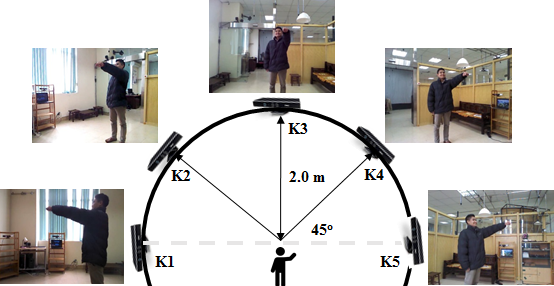
\includegraphics[width=0.8\linewidth]{figs/MICAGes1.png}
        \caption{Environment setup to capture MICAGes dataset.}
        %\vspace{-0.3cm}
        \label{Fig:MICAGes1}
    \end{figure}

    Twelve participants (08 males / 04 females) are voluntary to perform gestures one after another, each gesture three times.
    In the experiments of this thesis, only RGB information is concerned.
    Totally, the dataset contains 1620 (5 views $\times$ 9 gestures $\times$ 12 subjects $\times$ 3 times) dynamic hand gestures.
    Illustrations of segmented hand poses of a gesture are shown in Figure \ref{Fig:MICAGes2}.

    \begin{figure}[htbp]
        \centering
        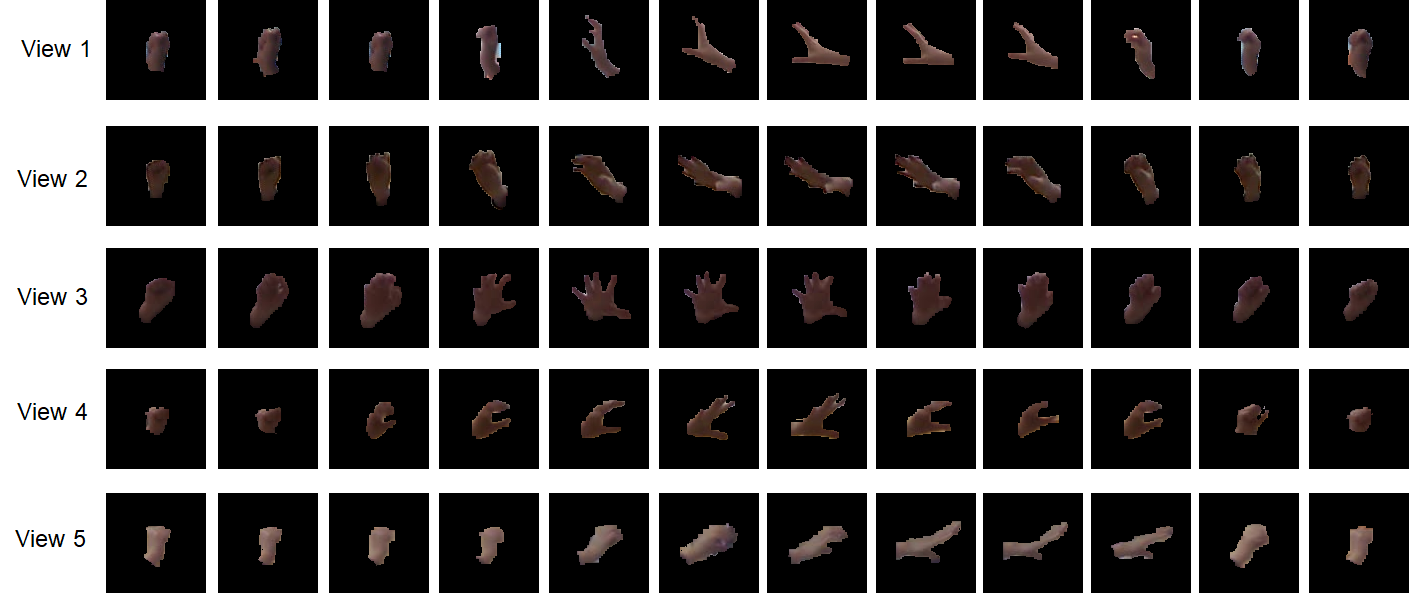
\includegraphics[width=0.9\linewidth]{figs/MICAGes2.png}
        \caption{Illustration of a gesture belonging to the $6^{th}$ class observed from 5 different views.}
        %\vspace{-0.3cm}
        \label{Fig:MICAGes2}
    \end{figure}


    %!TEX root = ../../main.tex

\section{Evaluation Protocol} \label{sec:protocol}
    The leave-one-actor out cross validation strategy represented in \cite{Stone1974} is employed and average accuracy (\%) are computed as means of comparison.
    In order to evaluate the proposed framework in terms of cross-view performance, it is further combined with cross-view validation.
    That means at a moment only two views are picked to evaluate, each consists of a train and a test part defined by the leave-one-actor out strategy.
    Apart from the proposed evaluation protocol, from now named ``\emph{protocol 1}'', another ``\emph{protocol 2}'' is assessed, which is regularly used in the literature.
    The main difference is in second protocol, the notation of train or test is omitted after feature extraction stage, every features samples from single view are included to train the multi-view metrics, then the classifier is fit on common features of one view and tested on common features of another view.
    It is noticed that the first evaluation protocol is more challenging because the in the second protocol, the constructed common space is already fit on the whole multi-view dataset. As a result, the later predictive models are trained and evaluated on features generated by a severely over-fitted projector. % Details about two evaluation protocols is presented in supplemental materials. 
    The difference between two protocols are illustrated in Figure \ref{Fig:ep}. 

    \begin{figure}[htbp]
      \centering
      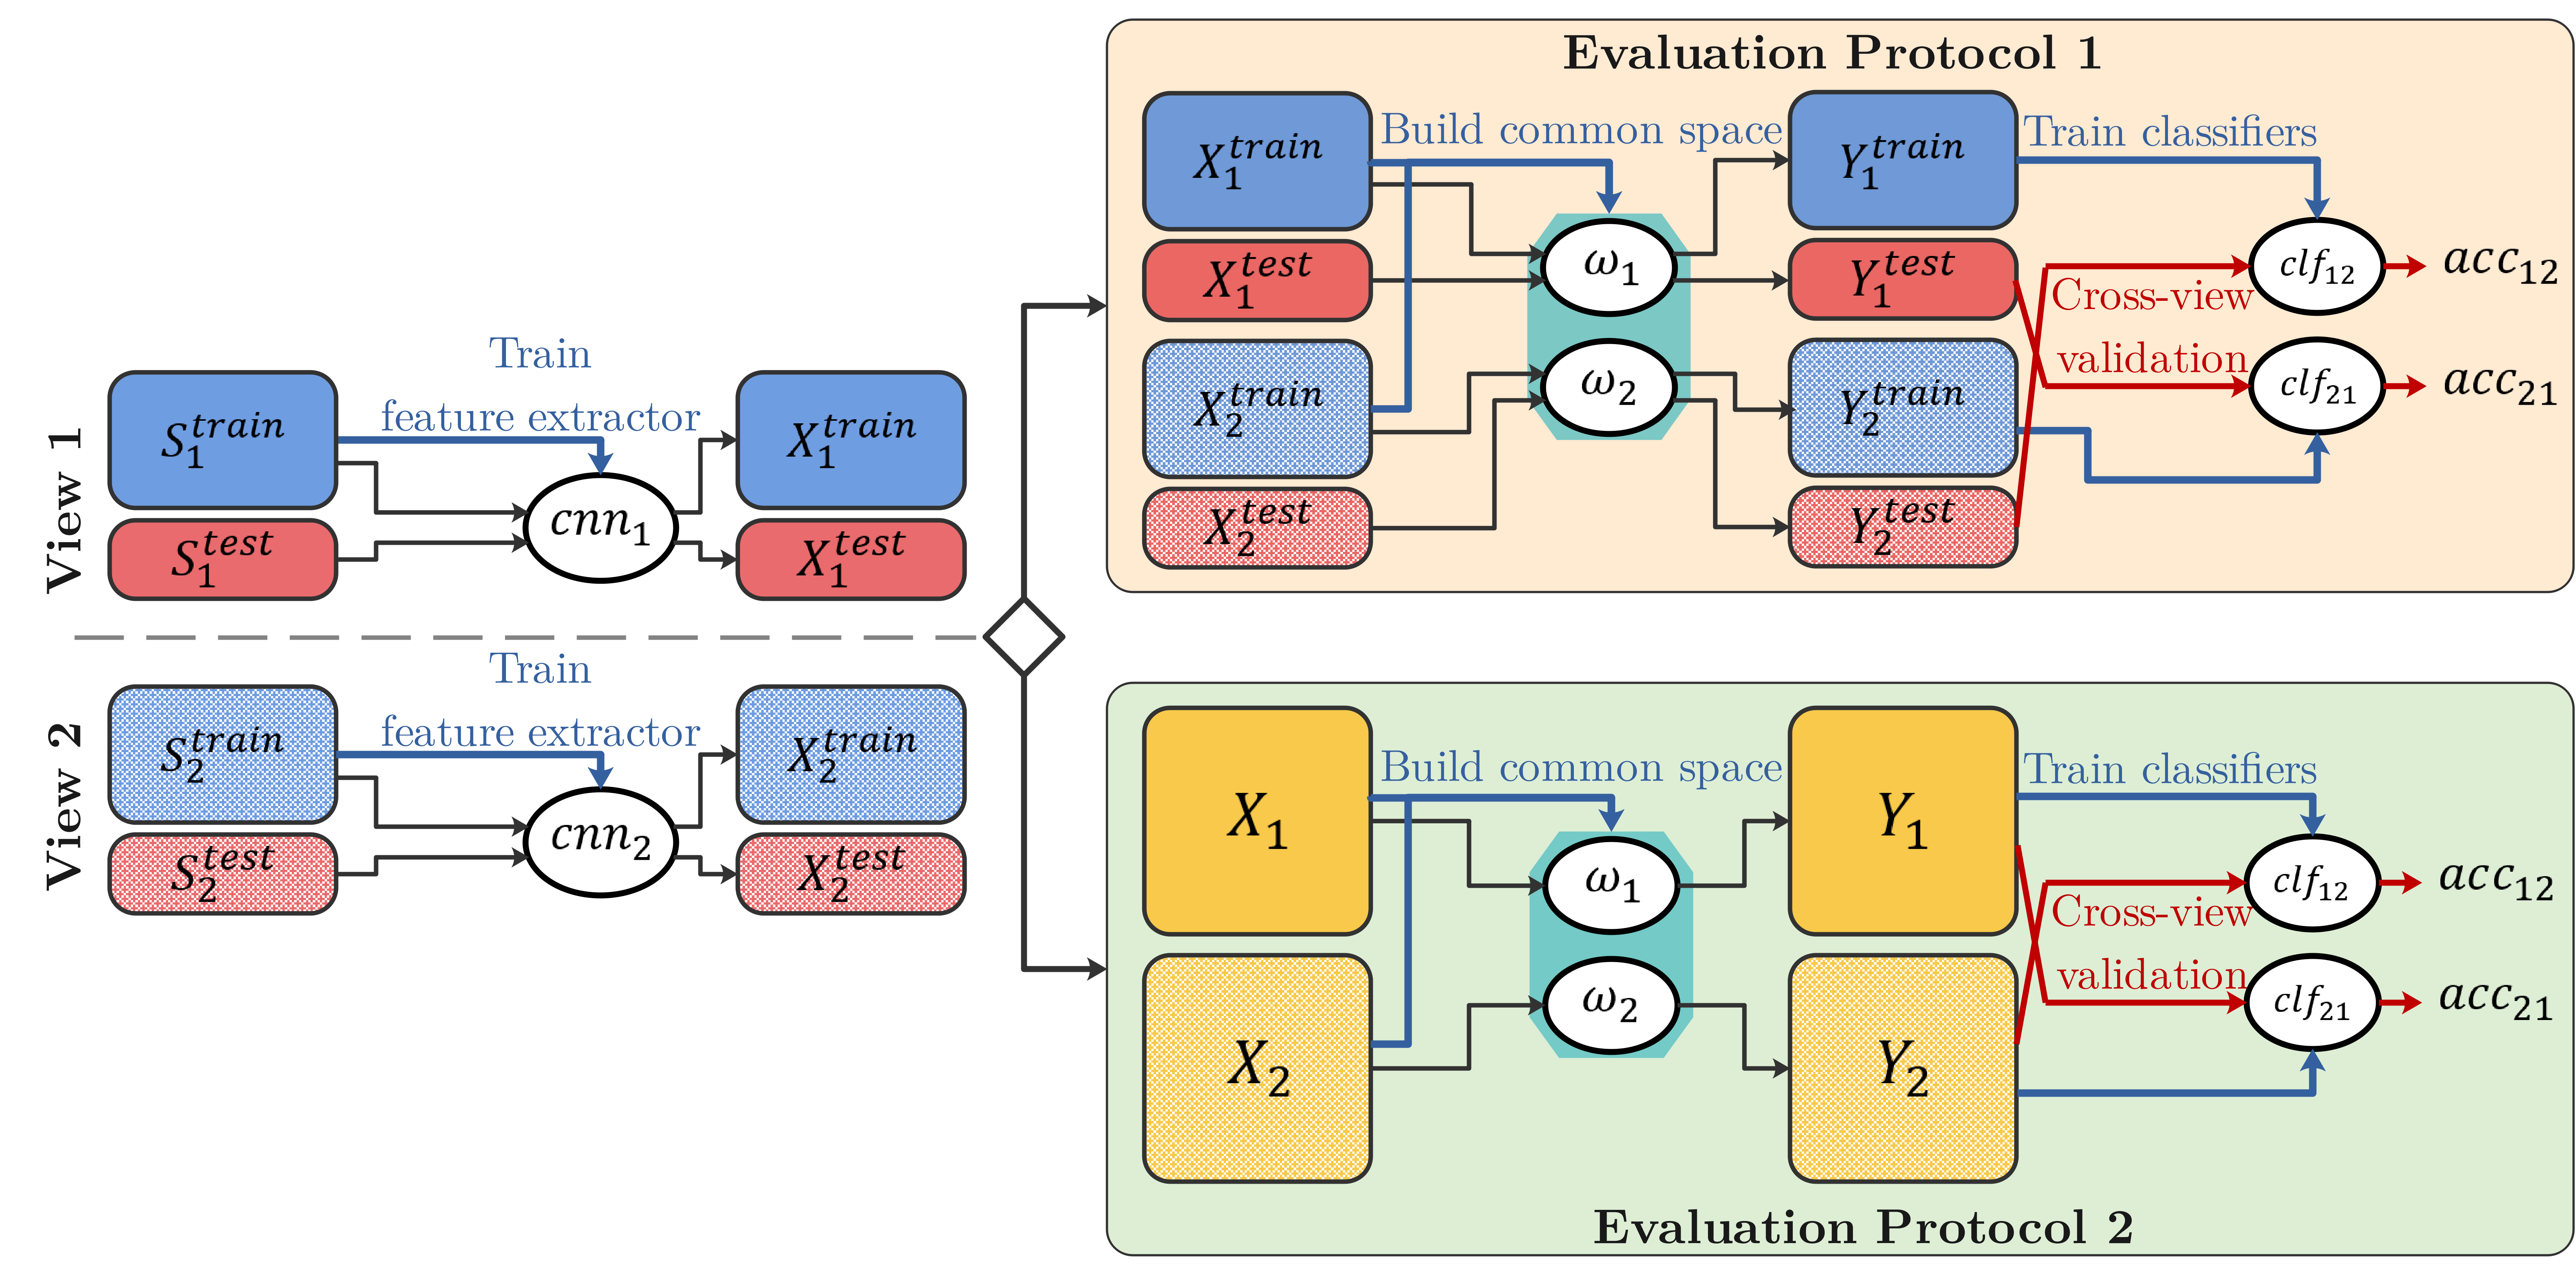
\includegraphics[width=1\linewidth]{figs/protocol.png}
      \caption{Two evaluation protocols used in experiments.}
        %\vspace{-0.3cm}
      \label{Fig:ep}
    \end{figure}
    The overall cross-view evaluation score is computed as average of all evaluation scores of each split, whose method of computation is described specifically in Figure \ref{Fig:ep}:
    \begin{equation}
        {acc}_{ij} = \frac{\sum_{k=1}^M {acc}^{(k)}_{ij}}{M}
    \end{equation}
    where M is the number of actors. Both protocols finally generate a cross-view accuracy matrix as follows:
    \begin{equation}
        \left[\begin{matrix}{acc}_{11}&{acc}_{12}&\cdots&{acc}_{1v}\\{acc}_{21}&{acc}_{22}&\cdots&{acc}_{2v}\\\vdots&\vdots&\ddots&\vdots\\{acc}_{v1}&{acc}_{v2}&\cdots&{acc}_{vv}\\\end{matrix}\right]
        \label{eq:multi-view_scores}
    \end{equation}
    For eager expression, let's define function $\operatorname{accuracy}\left(Y, \tilde{Y}\right)$ as the accuracy score when fitting a classifier on $Y$ features and evaluating its prediction on $\tilde{Y}$ features. Each cell can be expressed accordingly:
    \begin{align}
        {score}_{jr}^{\boldsymbol{protocol 1}} & =\left<\left\{\operatorname{accuracy}\left(Y_j^{train},Y_r^{test}\right)\middle|\ j,r=(1,..,v)\right\}\right> \\
        {score}_{jr}^{\boldsymbol{protocol 2}} & =\left<\left\{\operatorname{accuracy}\left(Y_j,Y_r\right)\middle|\ j,r=(1,..,v)\right\}\right>
    \end{align}

    \textbf{Multi-view strategy:} As MvDA and its variants can theoretically scale for an arbitrary number of views, in order to fairly compare the proposed algorithm with others that only apply for 2 views, I also experiment 2 different multi-view strategies. The key idea is that each strategy restricts the number of views participated in the training process of MvA algorithms.

    In ``\emph{multi-view}'' strategy, only one set of $W^*=\left\{{\omega}_1, {\omega}_2, ..., {\omega}_v\right\}$ is learnt and all separated view features are transformed $Y_j=\omega_j^TX_j,\ j=(1,...,v)$ before computation of accuracy.

    In ``\emph{cross-view}'' strategy, each cell ${score}_{jr}$ of \eqref{eq:multi-view_scores} must be calculated exclusively with the inclusion of only features of those views $j$ and $r$ (wihtout information from other views).
    Therefore, for each distinct combination $jk$, $W_{jr}^*=\left\{{\omega}_j, {\omega}_r\right\}$ is learnt to transform $X_j$ and $X_r$. The diagonal of \eqref{eq:multi-view_scores} is also ignored in this strategy.

    Since there are many scores generated by such extra complicated cross validation process when cycling through every actors, the final reported is average of all.
    Further, it is noticed that in existing works, the evaluation have been done mostly similar to the second evaluation protocol. Hence, in comparison with state of the art techniques, only the scores resulted from the second evaluation protocol are taken.

    %!TEX root = ../../main.tex

\section{Experimental Setup} \label{sec:experimental_setup}
    \subsection{Programming Environment and Libraries}
        The majority of my code implementation is written in Python, fueled by PyTorch \cite{NEURIPS2019_9015} deep learning framework.
        The framework offers powerful supports for matrix manipulation, automatic diffirentiation, accelerated training of deep neural networks on parallel computing platforms and flexibility to efficiently research new algorithmic approaches.
        The MvDA and MvDA-vc Matlab implementations are inherited from the repository published by \cite{kan2015multi} with slight modifications.
        The implementation of proposed pc-MvDA is published at \github{https://github.com/inspiros/pcmvda}.

    \subsection{Configurations}
        \paragraph{Feature extractors}
        All models are trained for 60 epoches with SGD optimizer, initial learning rate is 0.0003 and momentum is 0.9.
        The choosen pre-trained models are:
        \begin{itemize}
            \item{ResNet-50} model was pre-trained on ImageNet dataset and is available in subpackage \textit{torchvision.models} of PyTorch.
            \item{C3D} model was pre-trained on Sports-1M \cite{karpathy2014large} then fine-tuned on Kinetics dataset \cite{kay2017kinetics}. The model is implemented by \cite{VMZ} in Caffe2 deep learning framework, which was improved from original model presented in \cite{tran2015learning} by inserting Batch Normalization layers after each Convolution layer.
            \item{ResNet-50 3D} was pre-trained on Kinetics dataset and weights are given by \cite{hara2018can}.
        \end{itemize}

        \paragraph{Multi-view analysis algorithms}
        Output dimensions of both algorithms are 200. MvDA has no alterable parameter and $\lambda$ of view-consistency term in MvDA-vc is set to 0.03.
        For pc-MvDA, the hyperparameters are $\beta = 1$ and $q = 1$ and the optimizer utilized is Adam with initial learning rate set to 0.01, on each experiment trained 300 epochs.

        \paragraph{Classifier}
        For comparison with related methods, the final classifier used is kNN with $k = 1$.

    %!TEX root = ../../../main.tex

\section{Experimental Results and Discussions}
    %!TEX root = ../../../main.tex

\subsection{Experimental results on IXMAS dataset}
    \paragraph{1) Cross-view validation:} In this experiment, I train on data from one view (training view) and testing on data from another view (testing view) then compute the accuracies for two evaluation protocols. Table \ref{tab:cross_p1_ixmas} shows comparative results of using different deep features (C3D, ResNet-50 3D, ResNet-50 RNN, ResNet-50 TA, ResNet-50 AP) and multi-view discriminant analysis techniques (MvDA, MvDA-vc and my proposed pc-MvDA). 

    With the first evaluation protocol, the proposed pc-MvDA, when combined with deep features, gives mostly best accuracy for both evaluation protocols. With C3D features, accuracy by pc-MvDA (88.43\%) is 6.6\% higher than MvDA (81.84\%). pc-MvDA is even better than MvDA-vc (2.87\%). pc-MvDA achieved higher accuracy (about 6\% higher) than MvDA and MvDA-vc with ResNet-50 TA and ResNet-50 AP features. In average, pc-MvDA is 3.09\% higher than MvDA and 1.4\% higher than MvDA-vc.
    
    \begin{table}[htbp]
    \centering
    \caption{Cross-view recognition comparison on IXMAS dataset}
    \resizebox{0.8\textwidth}{!}{
    \begin{tabular}{|l|c|c|c|c|c|c|}
        \hline
        \multirow{2}{*}{Deep features}          & \multicolumn{3}{c|}{Protocol 1}   & \multicolumn{3}{c|}{Protocol 2}           \\ \cline{2-7} 
                                                & MvDA  & MvDA-vc & pc-MvDA         & MvDA  & MvDA-vc        & pc-MvDA          \\ \hline
        \multicolumn{1}{|c|}{C3D}               & 81.84 & 85.56   & \textbf{88.43}  & 96.54 & 99.29          & \textbf{99.98}   \\ \hline
        \multicolumn{1}{|c|}{ResNet-50 3D}      & 91.25 & 92.19   & \textbf{92.89}  & 97.30 & \textbf{99.73} & 99.65            \\ \hline
        \multicolumn{1}{|c|}{ResNet-50 RNN}     & 75.51 & 76.12   & \textbf{76.54}  & 99.99 & 99.71          & \textbf{100}     \\ \hline
        \multicolumn{1}{|c|}{ResNet-50 TA}      & 79.44 & 80.58   & \textbf{82.05}  & 99.33 & 99.34          & \textbf{99.84}   \\ \hline
        \multicolumn{1}{|c|}{ResNet-50 AP}      & 77.00 & 79.04   & \textbf{80.58}  & 99.68 & 99.81          & \textbf{99.92}   \\ \hline
    \end{tabular}}
    \label{tab:cross_p1_ixmas}
    \end{table}

    For the second evaluation protocol, pc-MvDA almost always keeps better performance compared to MvDA and MvDA-vc. The recognition accuracy scores obtained by both pc-MvDA and MvDA-vc are nearly 100\% for every kind of deep features. With C3D features and ResNet-50 3D features, pc-MvDA is 99.98\% and 99.65\%, which is 3.44\% and 2.35\% higher than the orginal MvDA (96.54\% and 97.3\%) respectively. In average, pc-MvDA is 1.31\% better than MvDA and 0.3\% better than MvDA-vc. 

    In terms of deep features, with the first evaluation protocol, ResNet-50 3D gives the best accuracy (92.89\%) following by C3D (88.43\%), ResNet-50 TA (82.05\%), ResNet-50 AP (80.58\%). The lowest accuracy obtained by ResNet-50 RNN is only 76.54\%. It shows that ResNet-50 3D produces the most discriminative feature space. %Table \ref{tab:cross_feature_ixmas} shows comparative results when using pc-MvDA method with different deep features regarding pairwise views. 

    \begin{table}[htbp]
    \centering
    \caption{Cross-view recognition results of different features on IXMAS dataset with pc-MvDA method. The result in the bracket are accuracies of using features C3D, ResNet-50 3D, ResNet-50 RNN, ResNet-50 TA, Restnet-50 AP respectively. Each row corresponds to training view (from view C0 to view C3). Each column corresponds to testing view (from view C0 to view C3)}
    \resizebox{\textwidth}{!}{\begin{tabular}{|c|c|c|c|c|}
        \hline
        \backslashbox{Training}{Testing} & C0 & C1 & C2 & C3 \\ \hline
        C0 & N/A & (90.7, \textbf{91.9}, 81.6, 84.6, 83.6) & (86.9, \textbf{93.9}, 78.0, 79.6, 78.1) & (89.9, \textbf{93.4}, 76.3, 82.8, 82.1) \\ \hline
        C1 & (86.6, \textbf{91.9}, 71.5, 81.1, 77.5) & N/A & (85.9, \textbf{94.2}, 78.6, 79.3, 80.3) & (88.9, \textbf{93.7}, 74.8, 82.3, 81.3) \\ \hline
        C2 & (87.6, \textbf{92.4}, 72.8, 81.8, 78.5) & (90.7, \textbf{91.7}, 80.6, 83.6, 82.6) & N/A & (89.4, \textbf{93.7}, 75.5, 82.3, 80.6) \\ \hline
        C3 & (87.6, \textbf{92.9}, 70.2, 82.1, 78.8) & (90.7, \textbf{91.2}, 81.6, 84.1, 82.8) & (86.4, \textbf{93.7}, 77.3, 80.6, 80.8) & N/A \\ \hline
    \end{tabular}}
    \label{tab:cross_feature_ixmas}
    \end{table}

    \paragraph{2) Multi-view validation} Table \ref{tab:ixmas_multi} shows multi-view recognition results. The conclusion is consistent with the case of cross-view evaluation: ResNet-50 3D is the best feature extractor. When it is combined with pc-MvDA, the framework gives the highest accuracy for the first protocol (92.82\%), following by C3D (88.19\%), ResNet-50 TA (81.49\%), ResNet-50 AP(80.43\%), and ResNet-50 RNN (76.47\%). Both MvA algorithms give similar accuracies for the second evaluation protocols (nearly 100\%). Again, pc-MvDA enhances the performance of MvDA by 2.43\% for the first protocol and 0.83\% for the second protocol. It only gives slightly better result than MvDA-vc (0.83\% for the first protocol and 0.74\% for the second protocol). 

    \begin{table}[htbp]
    \centering
    \caption{Multi-view recognition comparison on IXMAS dataset}
    \resizebox{0.7\textwidth}{!}{\begin{tabular}{|c|c|c|c|c|c|c|}
        \hline
        \multirow{2}{*}{Deep features}          & \multicolumn{3}{c|}{Protocol 1}   & \multicolumn{3}{c|}{Protocol2}                    \\ \cline{2-7} 
                                                & MvDA  & MvDA-vc & pc-MvDA         & MvDA           & MvDA-vc        & pc-MvDA         \\ \hline
        \multicolumn{1}{|c|}{C3D}               & 86.93 & 87.04   & \textbf{88.19}  & \textbf{99.99} & 99.44          & \textbf{99.98}  \\ \hline
        \multicolumn{1}{|c|}{ResNet-50 3D}      & 91.84 & 92.33   & \textbf{92.82}  & \textbf{100}   & 99.80          & 99,67           \\ \hline
        \multicolumn{1}{|c|}{ResNet-50 RNN}     & 72.44 & 75.95   & \textbf{76.47}  & 99.34          & \textbf{99.97} & \textbf{99.96}  \\ \hline
        \multicolumn{1}{|c|}{ResNet-50 TA}      & 76.74 & 81.01   & \textbf{81.49}  & 95.80          & 98.25          & \textbf{99.79}  \\ \hline
        \multicolumn{1}{|c|}{ResNet-50 AP}      & 79.28 & 78.93   & \textbf{80.43}  & \textbf{100}   & 98.11          & 99.85           \\ \hline
    \end{tabular}}
    \label{tab:ixmas_multi}
    \end{table}

    Figure \ref{fig:pc-MvDA_confusion_ixmas} compares the performance of feature extractors regarding each action class in multi-view evaluation scheme combined with the first evaluation protocol. There are clear margins between the performance of ResNet-50 3D and followed by C3D with other types of deep features, especially in harder actions (the first class to the third class and the eighth class to the eleventh class). These actions (check watch, cross arm, scratch head, wave, punch, kick, point) involve the most part static pose of the body and only movement of limbs, whereas other actions 4 - sit down, 5 - get up, 6 - turn around, 7 - walk and 12 - pickup include movement of the whole body and are easier to be recognized. This suggests that 3D convolution can better deal with small difference of movement in action images, which in turn generates a much more classification-ready feature space for latter stage of recognition.

    \begin{figure}[htbp]
        \centering
        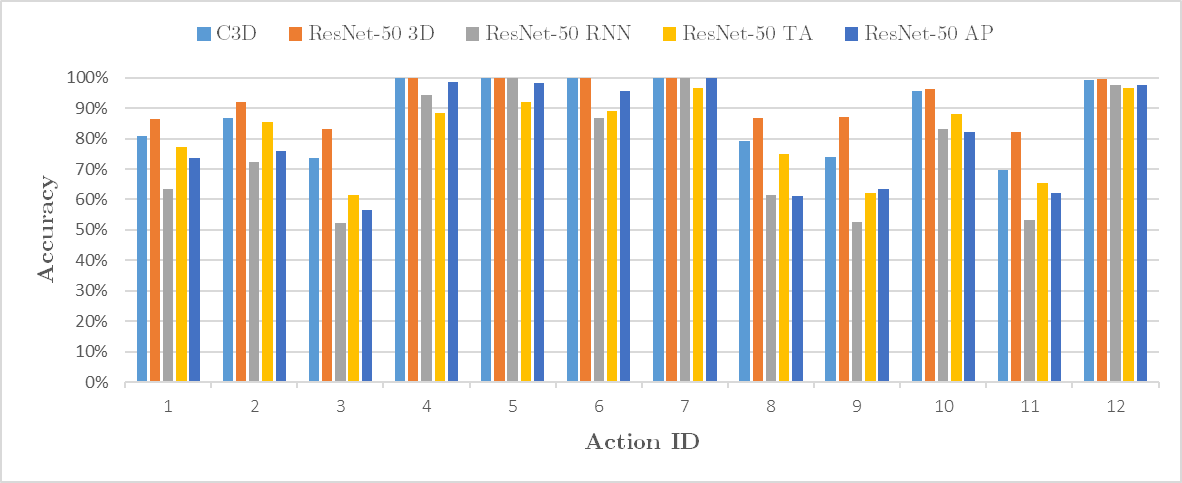
\includegraphics[width=0.8\linewidth]{figs/pc-MvDA_confusion_ixmas.png}
        \caption{Comparison of accuracy on each action class using different deep features combined with pc-MvDA on IXMAS dataset.}
        %\vspace{-0.3cm}
        \label{fig:pc-MvDA_confusion_ixmas}
    \end{figure}

    Table \ref{tab:sota_ixmas} compares the best combination of ResNet-50 3D and pc-MvDA with state-of-the-art frameworks. The comparison is for reference only because in other works, low-level hand-crafted video representation is used as private features and train-test strategy is leave-one-class out, which is not applicable to supervised deep feature extractors in this work. However, the results are still commensurable. % in circumstances where supervised approaches are adopted.
    % TODO - High priority

    \begin{table}[htbp]
    \centering
    \caption{Comparison of proposed methods with SOTA methods on IXMAS dataset according to the second evaluation protocol}
    \resizebox{0.7\textwidth}{!}{
    \begin{tabular}{|c|c|c|}
    \hline
    Methods                                                              & Cross-view & Multi-view \\ \hline
    Liu et al. \cite{liu2011cross}                                   & 76.32      & N/A       \\ \hline
    Zheng et al. \cite{zheng2012cross}                               & 95.1       & 99.32     \\ \hline
    Zheng et al. \cite{zheng2016cross}                               & 97.8       & 99.4      \\ \hline
    Kong et al. \cite{kong2017deeply}                                & 99.92      & 100       \\ \hline
    Ulhaq et al. \cite{ulhaq2017space}                               & 66.82      & 92.47     \\ \hline
    Zhang et al. \cite{zhang2018cross}                               & 84.1       & N/A        \\ \hline
    Liu et al. \cite{liu2018learning}                                & N/A        & 90.3     \\ \hline
    Liu et al. \cite{liu2018hierarchically}                          & 99.95      & 99.67     \\ \hline
    Proposed method (ResNet-50 3D + pc-MvDA)                     & 99.67      & 99.65       \\ \hline
    \end{tabular}}
    \label{tab:sota_ixmas}
    \end{table}

    %!TEX root = ../../../main.tex

\subsection{Experimental results on MuHAVi dataset}
    \paragraph{1) Cross-view validation:} Table.\ref{tab:muhavi_cross} illustrates cross-view recognition results. The proposed pc-MvDA consistently produces a better average accuracy of around 96.19\% for protocol 1, approximately 4.55\% and 1.51\% higher than that of MvDA (91.64\%) and MvDA-vc (94.67\%) respectively.

    \begin{table}[htbp]
    \centering
    \caption{Cross-view recognition comparison on MuHAVi dataset}
    \resizebox{0.8\textwidth}{!}{
    \begin{tabular}{|c|c|c|c|c|c|c|}
        \hline
        \multirow{2}{*}{Deep features}          & \multicolumn{3}{c|}{Protocol 1}   & \multicolumn{3}{c|}{Protocol 2}           \\ \cline{2-7} 
                                                & MvDA  & MvDA-vc & pc-MvDA         & MvDA  & MvDA-vc        & pc-MvDA          \\ \hline
        \multicolumn{1}{|c|}{C3D}               & 92.85 & 95.15   & \textbf{97.65}  & 98.95 & 99.76          & \textbf{100}     \\ \hline
        \multicolumn{1}{|c|}{ResNet-50 3D}      & 97.94 & 99.15   & \textbf{99.18}  & 96.77 & \textbf{99.94} & \textbf{99.94}   \\ \hline
        \multicolumn{1}{|c|}{ResNet-50 RNN}     & 95.54 & 95.14   & \textbf{96.18}  & 98.70 & 99.05          & \textbf{99.99}   \\ \hline
        \multicolumn{1}{|c|}{ResNet-50 TA}      & 85.80 & 88.95   & \textbf{91.12}  & 96.57 & 97.03          & \textbf{99.88}   \\ \hline
        \multicolumn{1}{|c|}{ResNet-50 AP}      & 86.09 & 94.98   & \textbf{96.82}  & 89.04 & 98.62          & \textbf{99.93}   \\ \hline
    \end{tabular}}
    \label{tab:muhavi_cross}
    \end{table}

    %Results in Table.\ref{tab:cross_feature_muhavi} show that our combination with ResNet-50 3D has the highest accuracies in almost every circumstances, even though both features coupled with our proposed pc-MvDA give satisfactory performance with all scores exceeding 91\%.

    \begin{table}[htbp]
    \centering
    \caption{Cross-view recognition results of different features on MuHAVi dataset with pc-MvDA method. The result in the bracket are accuracies of using features C3D, ResNet-50 3D, ResNet-50 RNN, ResNet-50 TA, ResNet-50 AP respectively. Each row corresponds to training view (from view C1 to view C7). Each column corresponds to testing view (from view C1 to view C7)}
    \resizebox{\textwidth}{!}{\begin{tabular}{|c|c|c|c|c|c|c|c|}
        \hline
        \backslashbox{Training}{Testing} & C1 & C2 & C3 & C4 & C5 & C6 & C7 \\ \hline
        C1 & N/A & \begin{tabular}{@{}c@{}} (96.1, \textbf{100}, 96.8, \\ 88.5, 98.5) \end{tabular} & \begin{tabular}{@{}c@{}} (98.6, \textbf{99.6}, 96.6, \\ 88.9, 96.3) \end{tabular} & \begin{tabular}{@{}c@{}} (98.6, \textbf{99.6}, 98.0, \\ 93.1, 98.2) \end{tabular} & \begin{tabular}{@{}c@{}} (97.7, \textbf{99.6}, 95.4, \\ 91.3, 96.1) \end{tabular} & \begin{tabular}{@{}c@{}} (97.7, \textbf{98.4}, 92.3, \\ 93.1, 96.3) \end{tabular} & \begin{tabular}{@{}c@{}} (98.2, \textbf{98.5}, 97.2, \\ 89.8, 97.1) \end{tabular} \\ \hline
        C2 & \begin{tabular}{@{}c@{}} (95.6, \textbf{99.0}, 95.2, \\ 91.3, 95.5) \end{tabular} & N/A & \begin{tabular}{@{}c@{}} (98.9, \textbf{99.6}, 96.9, \\ 90.3, 96.1) \end{tabular} & \begin{tabular}{@{}c@{}} (98.4, \textbf{99.6}, 97.6, \\ 92.6, 98.2) \end{tabular} & \begin{tabular}{@{}c@{}} (97.7, \textbf{99.6}, 95.4, \\ 90.9, 96.1) \end{tabular} & \begin{tabular}{@{}c@{}} (97.8, \textbf{98.4}, 92.7, \\ 93.6, 96.5) \end{tabular} & \begin{tabular}{@{}c@{}} (98.6, \textbf{99.0}, 97.4, \\ 90.6, 96.9) \end{tabular} \\ \hline
        C3 & \begin{tabular}{@{}c@{}} (96.1, \textbf{99.0}, 95.6, \\ 90.3, 95.1) \end{tabular} & \begin{tabular}{@{}c@{}} (97.0, \textbf{100}, 96.7, \\ 88.4, 97.8) \end{tabular} & N/A & \begin{tabular}{@{}c@{}} (98.1, \textbf{99.2}, 98.2, \\ 92.8, 98.2) \end{tabular} & \begin{tabular}{@{}c@{}} (97.9, \textbf{99.6}, 95.4, \\ 90.2, 95.6) \end{tabular} & \begin{tabular}{@{}c@{}} (97.9, \textbf{98.2}, 93.0, \\ 94.2, 96.5) \end{tabular} & \begin{tabular}{@{}c@{}} (97.8, \textbf{98.7}, 97.4, \\ 89.4, 97.6) \end{tabular} \\ \hline
        C4 & \begin{tabular}{@{}c@{}} (96.4, \textbf{98.8}, 95.4, \\ 89.6, 95.3) \end{tabular} & \begin{tabular}{@{}c@{}} (96.3, \textbf{100}, 96.6, \\ 91.0, 98.5) \end{tabular} & \begin{tabular}{@{}c@{}} (98.6, \textbf{99.6}, 97.3, \\ 89.5, 96.1) \end{tabular} & N/A & \begin{tabular}{@{}c@{}} (97.7, \textbf{99.4}, 95.6, \\ 91.3, 96.1) \end{tabular} & \begin{tabular}{@{}c@{}} (\textbf{98.4}, 98.0, 93.2, \\ 93.8, 95.6) \end{tabular} & \begin{tabular}{@{}c@{}} (97.7, \textbf{98.7}, 97.4, \\ 91.3, 96.7) \end{tabular} \\ \hline
        C5 & \begin{tabular}{@{}c@{}} (95.9, \textbf{99.0}, 95.6, \\ 91.3, 95.5) \end{tabular} & \begin{tabular}{@{}c@{}} (96.6, \textbf{100}, 97.1, \\ 89.9, 98.3) \end{tabular} & \begin{tabular}{@{}c@{}} (98.8, \textbf{99.4}, 96.8, \\ 90.7, 96.1) \end{tabular} & \begin{tabular}{@{}c@{}} (98.4, \textbf{99.6}, 98.0, \\ 92.1, 97.6) \end{tabular} & N/A & \begin{tabular}{@{}c@{}} (97.9, \textbf{98.2}, 93.4, \\ 94.4, 96.8) \end{tabular} & \begin{tabular}{@{}c@{}} (98.0, \textbf{98.7}, 96.9, \\ 89.0, 97.8) \end{tabular} \\ \hline
        C6 & \begin{tabular}{@{}c@{}} (95.8, \textbf{99.0}, 95.8, \\ 90.3, 95.0) \end{tabular} & \begin{tabular}{@{}c@{}} (97.0, \textbf{100}, 97.6, \\ 89.7, 98.5) \end{tabular} & \begin{tabular}{@{}c@{}} (98.8, \textbf{99.6}, 96.9, \\ 88.7, 96.1) \end{tabular} & \begin{tabular}{@{}c@{}} (98.4, \textbf{99.4}, 98.0, \\ 92.8, 98.2) \end{tabular} & \begin{tabular}{@{}c@{}} (97.5, \textbf{99.6}, 95.9, \\ 91.2, 95.5) \end{tabular} & N/A & \begin{tabular}{@{}c@{}} (98.2, \textbf{99.0}, 97.2, \\ 90.7, 97.4) \end{tabular} \\ \hline
        C7 & \begin{tabular}{@{}c@{}} (96.2, \textbf{98.8}, 95.7, \\ 91.5, 96.2) \end{tabular} & \begin{tabular}{@{}c@{}} (96.4, \textbf{100}, 97.5, \\ 90.3, 98.5) \end{tabular} & \begin{tabular}{@{}c@{}} (98.4, \textbf{99.0}, 97.3, \\ 90.0, 96.7) \end{tabular} & \begin{tabular}{@{}c@{}} (\textbf{98.8}, 98.8, 98.2, \\ 92.8, 98.0) \end{tabular} & \begin{tabular}{@{}c@{}} (97.5, \textbf{99.8}, 95.9, \\ 91.5, 95.9) \end{tabular} & \begin{tabular}{@{}c@{}} (\textbf{98.9}, 98.2, 92.8, \\ 93.9, 97.1) \end{tabular} & N/A \\ \hline
    \end{tabular}}
    \label{tab:cross_feature_muhavi}
    \end{table}

    \paragraph{2) Multi-view validation}: Table.\ref{tab:muhavi_multi} shows multi-view recognition results. The first protocol shows very close capability of MvDA-vc and pc-MvDA at 95.54\% and 95.83\% whereas MvDA is about 3\% behind at 92.7\%. For the second protocol, my variant exceeds MvDA by 2.21\% and MvDA-vc by 1.49\%. The near perfect results of the second protocol give us the same indication that it is not an inequitable method of comparison of MvL algorithms. 

    \begin{table}[htbp]
    \centering
    \caption{Multi-view recognition comparison on MuHAVi dataset}
    \resizebox{0.8\textwidth}{!}{
    \begin{tabular}{|c|c|c|c|c|c|c|}
        \hline
        \multirow{2}{*}{Deep features}          & \multicolumn{3}{c|}{Protocol 1}                   & \multicolumn{3}{c|}{Protocol2}            \\ \cline{2-7} 
                                                & MvDa           & MvDA-vc        & pc-MvDa         & MvDa           & MvDA-vc & pc-MvDa        \\ \hline
        \multicolumn{1}{|c|}{C3D}               & 81.80          & 96.05          & \textbf{97.37}  & 88.39          & 99.61   & \textbf{100}   \\ \hline
        \multicolumn{1}{|c|}{ResNet-50 3D}      & 99.07          & 99.12          & \textbf{99.15}  & \textbf{99.98} & 99.96   & 99.89          \\ \hline
        \multicolumn{1}{|c|}{ResNet-50 RNN}     & \textbf{96.18} & 95.55          & 95.97           & \textbf{100}   & 99.00   & 99.98          \\ \hline
        \multicolumn{1}{|c|}{ResNet-50 TA}      & \textbf{90.45} & 89.73          & 90.22           & \textbf{99.92} & 98.17   & 99.72          \\ \hline
        \multicolumn{1}{|c|}{ResNet-50 AP}      & 96.01          & \textbf{96.75} & 96.42           & \textbf{100}   & 95.13   & 99.68          \\ \hline
    \end{tabular}}
    \label{tab:muhavi_multi}
    \end{table}

    Figure.\ref{fig:pc-MvDA_confusion_muhavi} compares the performance of feature extractors regarding each action class in multi-view evaluation scheme combined with protocol 1. For this dataset, ResNet-50 3D persistently yields out-standing performance while ResNet-50 TA has the worst recognition rates in all action classes.

    \begin{figure}[htbp]
        \centering
        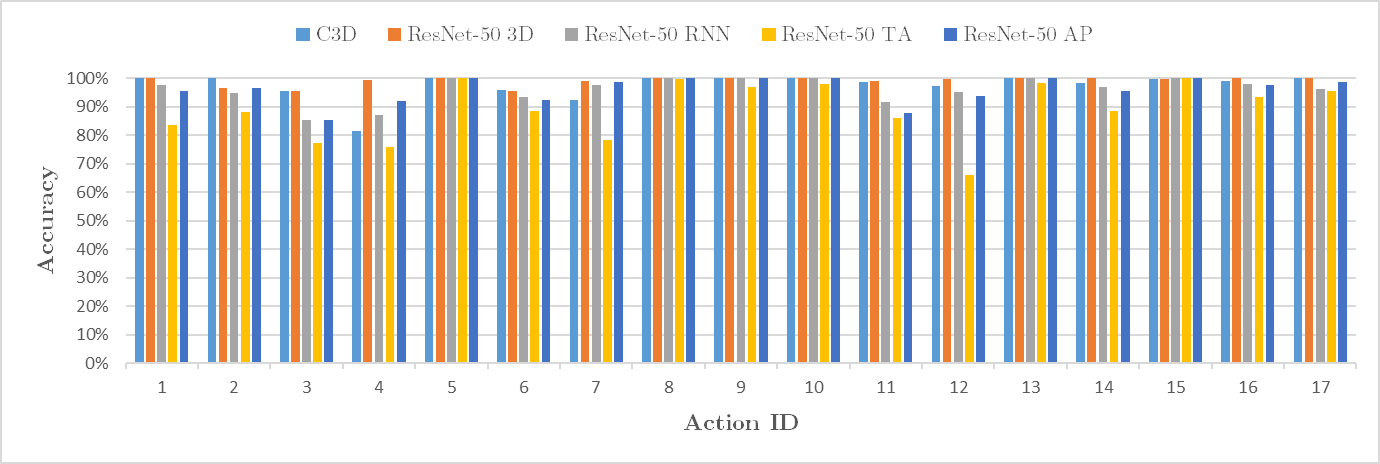
\includegraphics[width=1.0\linewidth]{Figs/pc-MvDA_confusion_muhavi.png}
        \caption{Comparison of accuracy on each action class using different deep features combined with pc-MvDA.}
        %\vspace{-0.3cm}
        \label{fig:pc-MvDA_confusion_muhavi}
    \end{figure}

    Table.\ref{tab:sota_muhavi} compares the best investigated combination of ResNet-50 3D and pc-MvDA with state-of-the-art frameworks. The comparison is for reference only because of aforementioned difference in setup of number of views and cross validation scheme.

    \begin{table}[htbp]
    \centering
    \caption{Comparison of the proposed methods with SOTA methods on MuHAVi dataset according to the second evaluation protocol.}
    \resizebox{0.7\textwidth}{!}{
    \begin{tabular}{|c|c|c|}
    \hline
    Methods                                                   & Cross-view & Multi-view \\ \hline
    Wu et al. \cite{wu2012view}                               & N/A       & 94.5     \\ \hline
    Zheng et al. \cite{zheng2016cross}                        & 94.88     & 99.8     \\ \hline
    Liu et al. \cite{liu2018learning}                         & N/A       & 91.2     \\ \hline
    Liu et al. \cite{liu2018hierarchically}                   & 99.91     & 99.8     \\ \hline
    Proposed method (ResNet-50 3D + pc-MvDA) \protect\footnotemark              & 99.90     & 99.88    \\ \hline
    \end{tabular}}
    \label{tab:sota_muhavi}
    \end{table}
    \footnotetext{Results when choosing only 4 views Camera 1, Camera 3, Camera 4 and Camera 6 following the other works.}

    %!TEX root = ../../../main.tex

\subsection{Experimental results on MICAGes dataset}

    \paragraph{1) Cross-view validation:} It can be seen in Table.\ref{tab:mica_cross} that pc-MvDA outperforms in almost every cases. With the first protocol, the norm accuracy of pc-MvDA of 74.52\% surpasses that of MvDA-vc (72.12\%) by 2.4\% and that of MvDA (64.94\%) by a large margin of 9.58\%. Especially in case of C3D features, the proposed algorithm achieved 90.2\% recognition rate whereas MvDA returns only 67.13\%.

    \begin{table}[htbp]
    \centering
    \caption{Cross-view recognition comparison on MICAGes dataset.}
    \resizebox{0.8\textwidth}{!}{
    \begin{tabular}{|c|c|c|c|c|c|c|}
        \hline
        \multirow{2}{*}{Deep features}          & \multicolumn{3}{c|}{Protocol 1}          & \multicolumn{3}{c|}{Protocol 2}            \\ \cline{2-7} 
                                                & MvDA  & MvDA-vc        & pc-MvDA         & MvDA  & MvDA-vc        & pc-MvDA           \\ \hline
        \multicolumn{1}{|c|}{C3D}               & 67.13 & 85.98          & \textbf{90.20}  & 93.74 & 99.80          & \textbf{100}      \\ \hline
        \multicolumn{1}{|c|}{ResNet-50 3D}      & 94.91 & 95.25          & \textbf{95.62}  & 97.43 & \textbf{99.97} & 99.79             \\ \hline
        \multicolumn{1}{|c|}{ResNet-50 RNN}     & 58.01 & 61.64          & \textbf{64.13}  & 100   & 100            & 100               \\ \hline
        \multicolumn{1}{|c|}{ResNet-50 TA}      & 53.58 & \textbf{59.55} & 58.62           & 96.70 & 99.48          & \textbf{99.83}    \\ \hline
        \multicolumn{1}{|c|}{ResNet-50 AP}      & 51.07 & 58.19          & \textbf{64.04}  & 99.73 & \textbf{99.99} & 99.89             \\ \hline
    \end{tabular}}
    \label{tab:mica_cross}
    \end{table}

    %Table.\ref{tab:cross_feature_mica} compares all types of deep features regarding accuracy of the proposed algorithm. 
    The top ranking of features applies identically and radically proves the superiority of 3D convolution based clip-level feature extraction in video recognition: ResNet-50 3D at 95.62\% and C3D at 90.2\%. The rest are ResNet-50 RNN (64.13\%), ResNet-50 AP (64.04\%) and ResNet-50 TA (58.62\%). For the second protocol, MvDA-vc (99.85\%) and pc-MvDA (99.9\%) are nearly even in performance while MvDA achieved 97.52\%.

    \begin{table}[htbp]
    \centering
    \caption{Cross-view recognition results of different features on MICAGes dataset with pc-MvDA method. The result in the bracket are accuracies of using features C3D, ResNet-50 3D, ResNet-50 RNN, ResNet-50 TA, RestNet-50 AP respectively. Each row corresponds to training view (from view K1 to view K5). Each column corresponds to testing view (from view K1 to view K5).}
    \resizebox{\textwidth}{!}{\begin{tabular}{|c|c|c|c|c|c|}
        \hline
        \backslashbox{Training}{Testing} & K1 & K2 & K3 & K4 & K5 \\ \hline
        K1 & N/A & \begin{tabular}{@{}c@{}} (92.9, \textbf{95.5}, 69.4, \\ 63.9, 65.1) \end{tabular} & \begin{tabular}{@{}c@{}} (93.7, \textbf{98.0}, 79.1, \\ 75.8, 74.7) \end{tabular} & \begin{tabular}{@{}c@{}} (90.5, \textbf{97.6}, 64.5, \\ 68.8, 70.8) \end{tabular} & \begin{tabular}{@{}c@{}} (89.2, \textbf{92.6}, 56.0, \\ 43.7, 58.2) \end{tabular} \\ \hline       
        K2 & \begin{tabular}{@{}c@{}} (84.7, \textbf{94.6}, 51.3, \\ 41.4, 53.7) \end{tabular} & N/A & \begin{tabular}{@{}c@{}} (94.6, \textbf{97.6}, 78.9, \\ 75.4, 77.5) \end{tabular} & \begin{tabular}{@{}c@{}} (91.3, \textbf{97.6}, 64.4, \\ 68.5, 68.0) \end{tabular} & \begin{tabular}{@{}c@{}} (87.4, \textbf{92.7}, 56.1, \\ 42.0, 55.6) \end{tabular} \\ \hline       
        K3 & \begin{tabular}{@{}c@{}} (87.5, \textbf{94.9}, 51.9, \\ 43.6, 52.7) \end{tabular} & \begin{tabular}{@{}c@{}} (93.0, \textbf{95.5}, 70.1, \\ 64.7, 63.4) \end{tabular} & N/A & \begin{tabular}{@{}c@{}} (90.0, \textbf{97.6}, 63.2, \\ 62.6, 67.5) \end{tabular} & \begin{tabular}{@{}c@{}} (88.9, \textbf{92.2}, 57.2, \\ 41.8, 56.6) \end{tabular} \\ \hline       
        K4 & \begin{tabular}{@{}c@{}} (86.7, \textbf{94.7}, 50.8, \\ 48.9, 54.9) \end{tabular} & \begin{tabular}{@{}c@{}} (90.2, \textbf{95.5}, 71.5, \\ 68.2, 61.8) \end{tabular} & \begin{tabular}{@{}c@{}} (92.5, \textbf{98.0}, 81.0, \\ 76.0, 74.4) \end{tabular} & N/A & \begin{tabular}{@{}c@{}} (89.7, \textbf{92.3}, 54.3, \\ 44.9, 56.6) \end{tabular} \\ \hline       
        K5 & \begin{tabular}{@{}c@{}} (84.9, \textbf{94.9}, 48.4, \\ 41.5, 57.9) \end{tabular} & \begin{tabular}{@{}c@{}} (90.4, \textbf{95.5}, 72.6, \\ 64.1, 65.7) \end{tabular} & \begin{tabular}{@{}c@{}} (94.0, \textbf{97.8}, 79.1, \\ 72.5, 76.3) \end{tabular} & \begin{tabular}{@{}c@{}} (91.9, \textbf{97.3}, 62.7, \\ 64.1, 69.0) \end{tabular} & N/A \\ \hline
    \end{tabular}}
    \label{tab:cross_feature_mica}
    \end{table}

    \paragraph{2) Multi-view validation}: The multi-view recognition results in Table.\ref{tab:mica_multi} shows an almost alike trend for both protocols. In general, pc-MvDA is 8.95\% and 0.72\% higher in accuracy for protocol 1, and 2.75\% and 0.04\% for protocol 2, in comparison with MvDA and MvDA-pc respectively.

    % TODO
    In virtually every experiments of MICAGes and two earlier benchmark datasets, the proposed extension is superior. The average accuracies of pc-MvDA is, in comparison on protocol 1 (and protocol 2 resp.), 5.29\% (1.21\% resp.) higher than MvDA, 1.21\% (0.62\% resp.) better than MvDA-vc. Despite not being as intuitive and straightly intelligible as pairwise-covariance, the multi-view resemblance added in MvDA-vc achieved nearly the performance of pc-MvDA. However, this view-consistency can be easily splitted into pairwise terms and intergrated into the objective of pc-MvDA in future works for further analysis.

    \begin{table}[htbp]
    \centering
    \caption{Multi-view recognition comparison on MICAGes dataset.}
    \resizebox{0.8\textwidth}{!}{
    \begin{tabular}{|c|c|c|c|c|c|c|}
        \hline
        \multirow{2}{*}{Deep features}          & \multicolumn{3}{c|}{Protocol 1}          & \multicolumn{3}{c|}{Protocol2}                     \\ \cline{2-7} 
                                                & MvDA  & MvDA-vc        & pc-MvDA         & MvDA           & MvDA-vc       & pc-MvDA           \\ \hline
        \multicolumn{1}{|c|}{C3D}               & 68.31 & 87.70          & \textbf{89.99}  & 88.79          & 99.54         & \textbf{100}      \\ \hline
        \multicolumn{1}{|c|}{ResNet-50 3D}      & 95.32 & 95.26          & \textbf{95.54}  & \textbf{100}   & 99.96         & 99.80             \\ \hline
        \multicolumn{1}{|c|}{ResNet-50 RNN}     & 57.50 & 63.05          & \textbf{63.83}  & 99.90          & \textbf{100}  & 99.97             \\ \hline
        \multicolumn{1}{|c|}{ResNet-50 TA}      & 54.43 & \textbf{61.46} & 58.25           & 96.72          & 99.49         & \textbf{99.69}    \\ \hline
        \multicolumn{1}{|c|}{ResNet-50 AP}      & 50.93 & 60.20          & \textbf{63.66}  & \textbf{99.99} & 99.93         & 99.67             \\ \hline
    \end{tabular}}
    \label{tab:mica_multi}
    \end{table}

    In addition to the same propensity shown, MICAGes also reveals the robustness of 3D convolution to generate fine clustered private feature space because this dataset contains exclusively hand gestures, which take part in a relatively small region of the captured videos. ResNet-50 3D and C3D are predominant for discriminant common space construction and classification and distances other features (Figure \ref{fig:pc-MvDA_confusion_mica}).

    \begin{figure}[htbp]
        \centering
        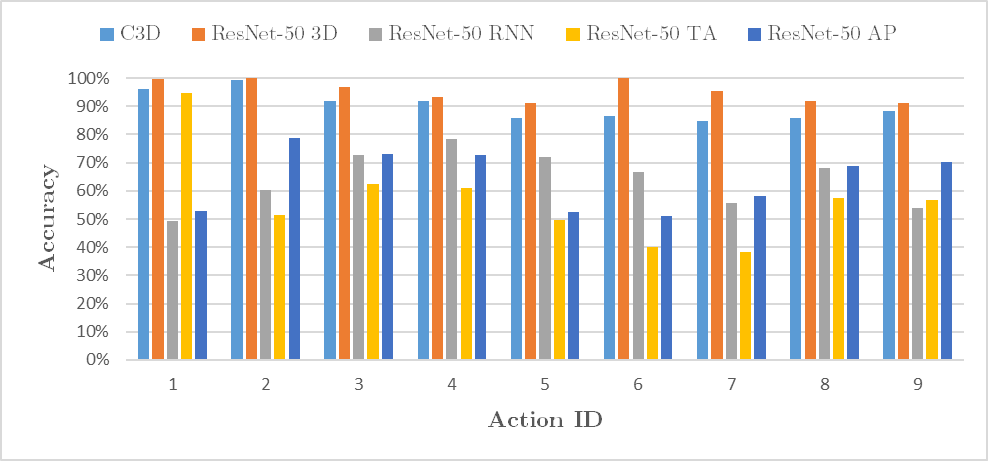
\includegraphics[width=0.8\linewidth]{figs/pc-MvDA_confusion_mica.png}
        \caption{Comparison of accuracy on each action class using different deep features combined with pc-MvDA on MICAGes dataset.}
        %\vspace{-0.3cm}
        \label{fig:pc-MvDA_confusion_mica}
    \end{figure}

    To better study the behavior of investigated multi-view analysis algorithms, t-SNE embedding of original private spaces, MvDA and pc-MvDA common space generated by protocol 1 are plotted in Figure \ref{fig:mica-tsne}. In these scatter plots, colors denote action classes, shapes as different views and train/test data are distinguished by border type. They explicitly denotes the surpassing capability of the proposed algorithm in finding a common space with prominent extra-class discrepancy. The data samples involved in training process are generally clustered in compact and separated blobs while testing data samples dissolve nearby. The better convergence of pc-MvDA compared to the baseline is usually only visible for harder features, whereas with the inputs of ResNet-50 3D features, which are already highly discriminated in private spaces, the improvement of pc-MvDA is negligible. Note that these illustrations of t-SNE embedding do not strictly depict an identical distribution of data.

    \begin{figure}[htbp]
        \centering
        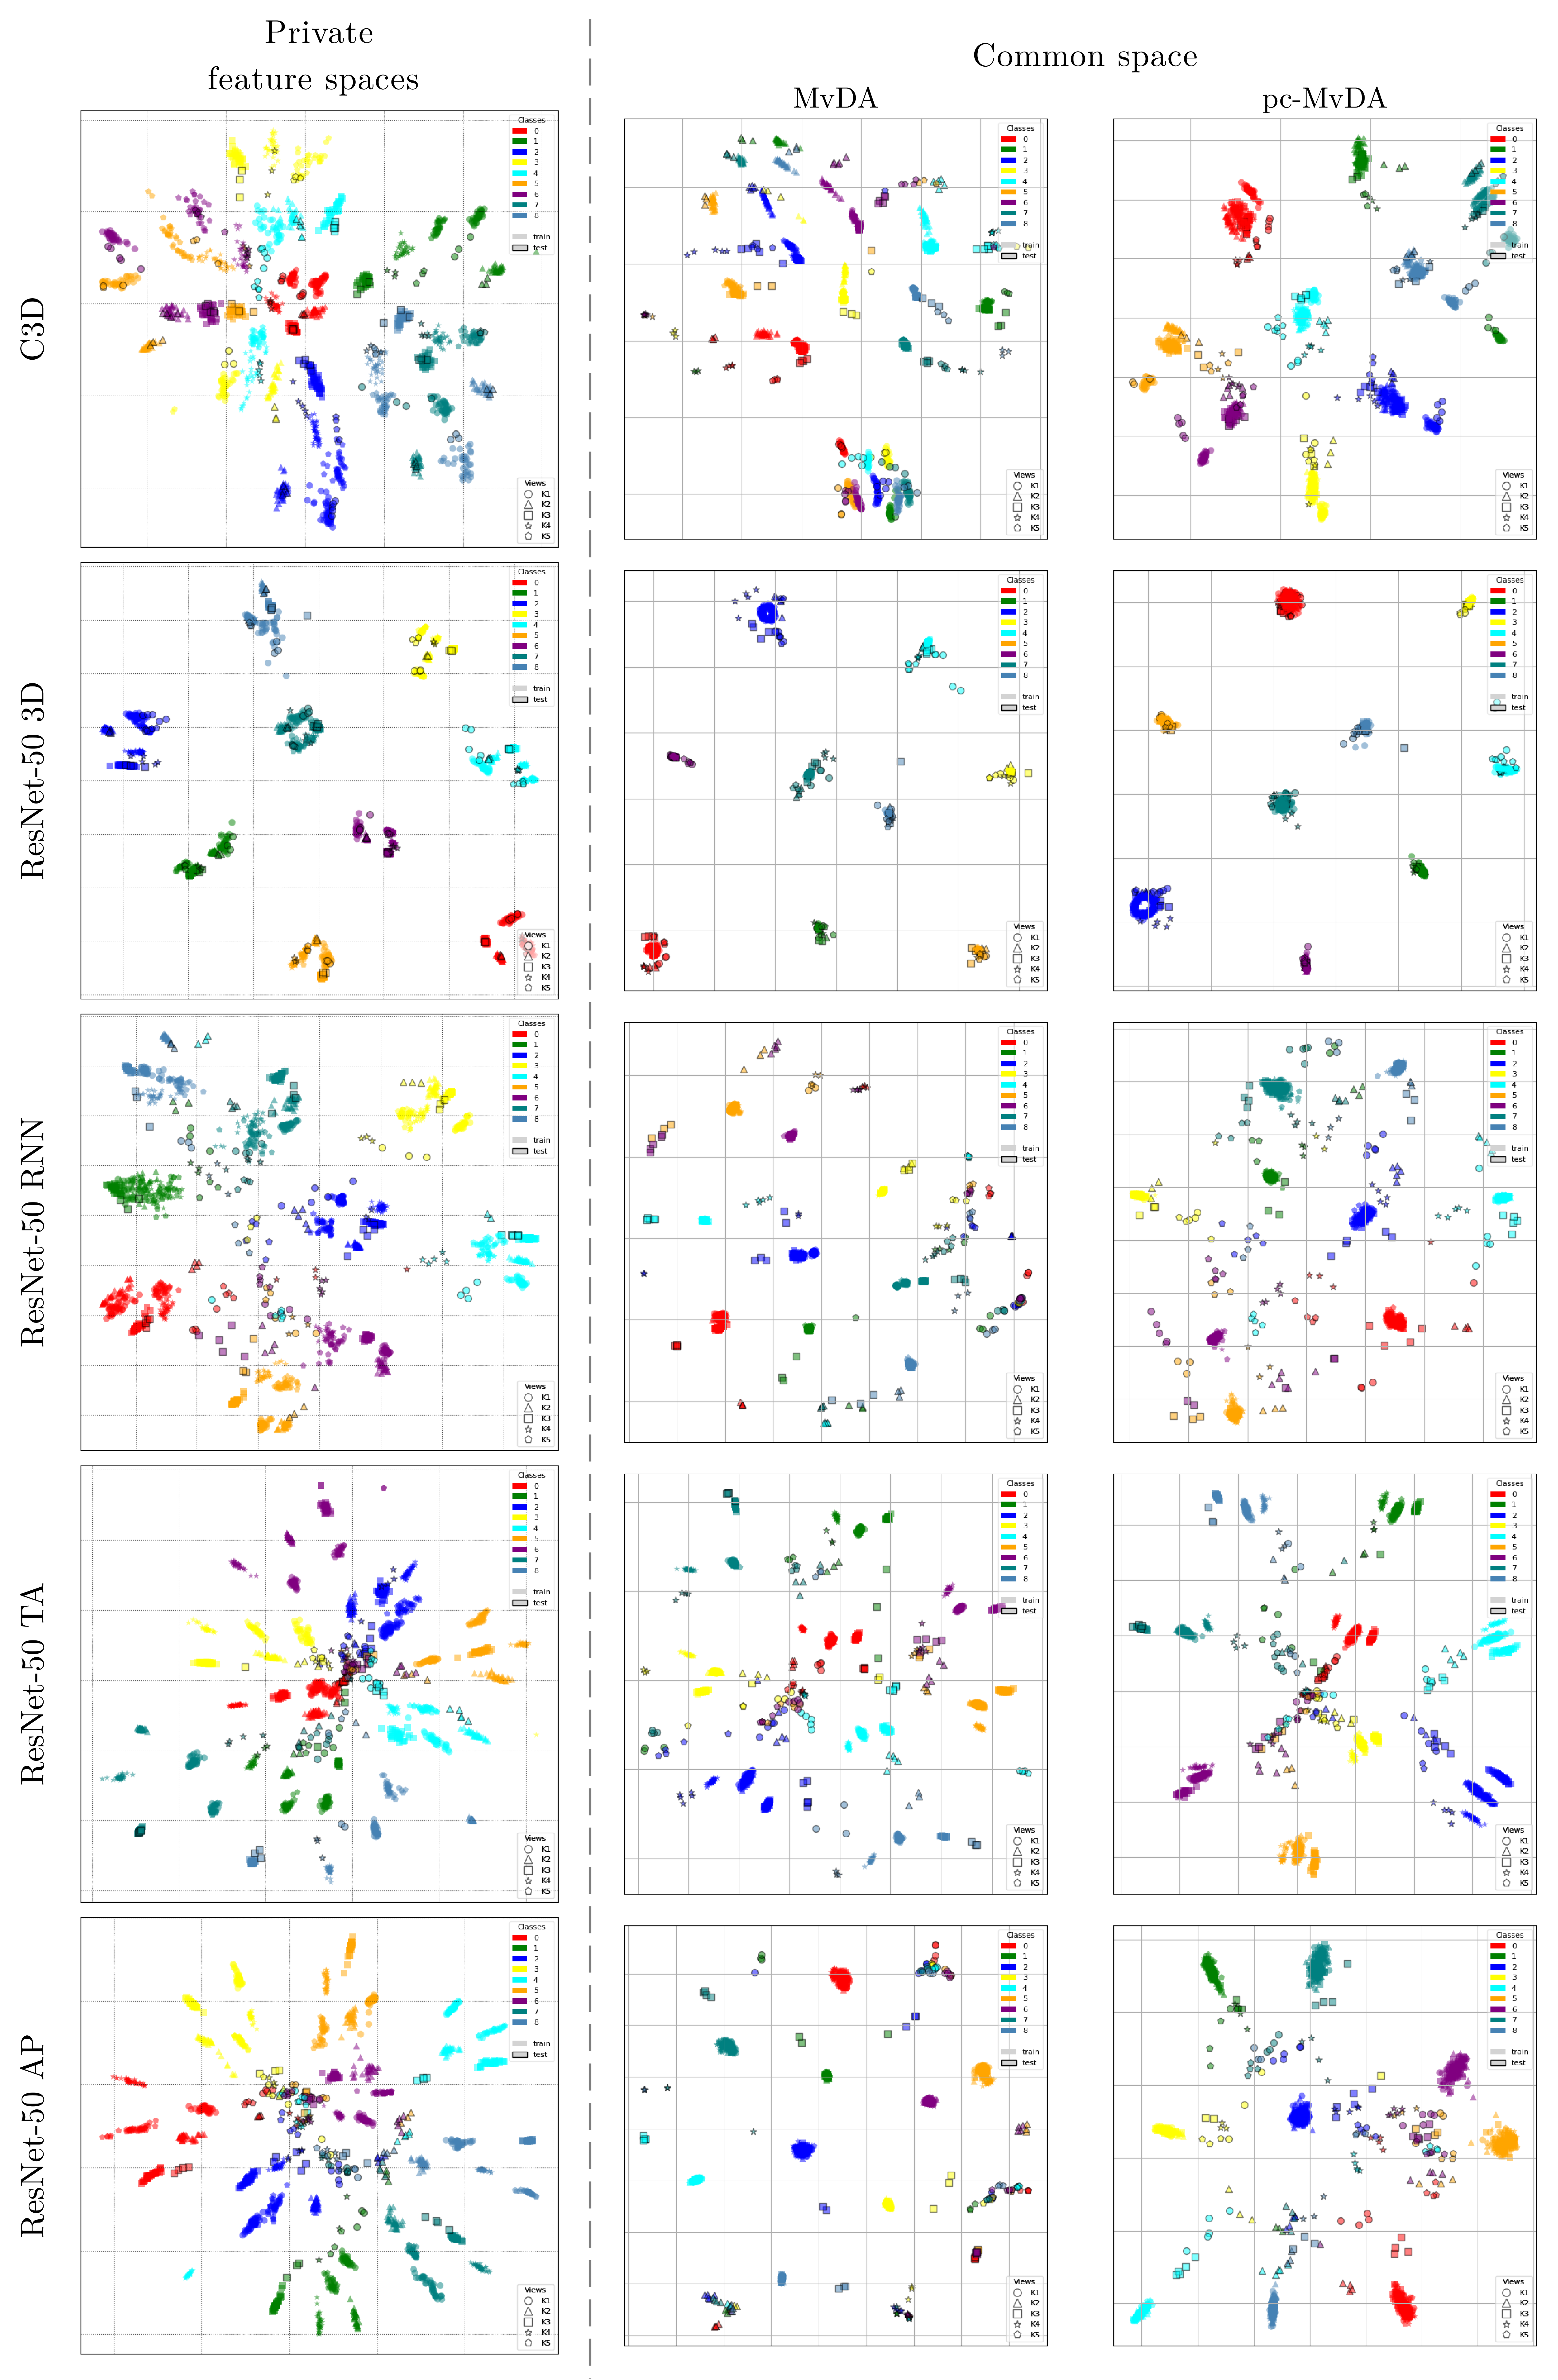
\includegraphics[width=1\linewidth, height=0.6\pdfpageheight, keepaspectratio=false]{figs/mica-tsne.png}
        \caption{First column: private feature spaces stacked and embedded together in a same coordinate system; Second column: MvDA common space; Third column: pc-MvDA common space.}
        %\vspace{-0.3cm}
        \label{fig:mica-tsne}
    \end{figure}



    \section{Summary}
        The experiments conducted indicates that the framework could achieve competitive results.
        The second evaluation protocol is shown to be less equitable for multi-view analysis algorithms compared to the first evaluation protocol represented in this thesis.
        Overall, the proposed pc-MvDA also achieved amelioration in almost every cases compared to baseline MvDA by a 5.29\% margin in terms of average accuracy.

    %!TEX root = ../../main.tex

\chapter{Conclusion} \label{chap:conclusion}
    %!TEX root = ../../main.tex

\section{Accomplishments}
    This thesis has presented a novel framework for human action recognition.
    The framework integrates various successful deep features with multi-view discriminant analysis to deal with cross-view human action recognition.
    In particular, five deep models have been utilized: ResNet with three pooling techniques; ResNet-3D and C3D.
    These deep features have been universally used for action recognition from a common view but rarely utilized for evaluating cross-view HAR.
    Besides, three variations of multi-view discriminant analysis: the original MvDA, MvDA with view consistency (MvDA-vc) and my proposed pairwise-covariance MvDA (pc-MvDA) have been investigated.
    Multi-view analysis algorithms have been successfully deployed for cross-view recognition of static images but never applied for spatio-temporal features.
    The experiments show that the proposed algorithm achieved highest average accuracy (5.29\% higher than MvDA and 1.21\% higher than MvDA-vc).
    % In addition, ResNet-50 3D gives the best overall HAR accuracy for both cross-view and multi-view evaluation protocols.
    % It concludes that the combination of deep features with pc-MvDA is suitable and feasible to deploy the proposed framework in practical applications. 

    %!TEX root = ../../main.tex

\section{Drawbacks} \label{sec:drawbacks}
    The overall framework is not end-to-end trainable.
    The proposed pc-MvDA is a batch algorithm, in effect, it is essential to process whole training dataset at once to compute class means at each optimization step.
    This makes pc-MvDA unsuitable to be a loss function that trains multiple large-scale neural networks concurrently, especially when input data is 3-dimensional spatio-temporal tensors.
    
    %!TEX root = ../../main.tex

\section{Future Works}



    \cleardoublepage
    \footnotesize
    \ihead[]{Bibliography}
    \bibliography{main}
    \normalsize

\end{document}
